
\documentclass{BscUS}
\usepackage{setspace}
\usepackage{graphicx}
\usepackage{polski}
\usepackage{subfig}
\usepackage[utf8]{inputenc}
\usepackage{verbatim}
\usepackage{fourier}
\usepackage[T1]{fontenc}
\usepackage{enumitem}
\setitemize{noitemsep,topsep=0pt,parsep=0pt,partopsep=0pt}
\usepackage{float}
\usepackage{amsmath}
\usepackage{gensymb}
\usepackage{physics}
\usepackage{siunitx}
\usepackage{nameref}
\usepackage{listing}
\usepackage{listings}
\usepackage{indentfirst}
\usepackage{color}

\usepackage{array}
\usepackage[all]{nowidow}
 \usepackage{multirow}
 \usepackage[table,xcdraw]{xcolor}
 
 \usepackage{epstopdf} 
 \usepackage{epsfig}

\usepackage{afterpage}

\newcommand\blankpage{%
    \null
    \thispagestyle{empty}%
    \newpage}
\addtocounter{page}{-1}%
\usepackage{fancyvrb}
\DefineVerbatimEnvironment{packet}{Verbatim}{xleftmargin=40mm,baselinestretch=1,samepage=true}
\DefineVerbatimEnvironment{code}{Verbatim}{xleftmargin=36pt,samepage=true,tabsize=4}

\usepackage{fancyhdr}
\pagestyle{fancy}

\fancyhf{}
\fancyhead[RE,LO]{\leftmark}
\fancyhead[LE,RO]{\thepage}
\renewcommand{\headrulewidth}{1pt} 

%%\renewcommand{\labelenumi}{\Roman{enumi}}

\graphicspath{{img}}

\title{Opracowanie systemu szybkiego przesyłania danych z wykorzystaniem standardu USB}

\author{Łukasz Pawlik}
\promoter{dr inż. Bartosz Mindur}
\where{Kraków}
\when{2016}


\definecolor{mygreen}{rgb}{0,0.6,0}
\definecolor{mygray}{rgb}{0.5,0.5,0.5}
\definecolor{mymauve}{rgb}{0.58,0,0.82}

\lstset{ %
  backgroundcolor=\color{white},   % choose the background color; you must add \usepackage{color} or \usepackage{xcolor}
  basicstyle=\footnotesize,        % the size of the fonts that are used for the code
  breakatwhitespace=false,         % sets if automatic breaks should only happen at whitespace
  breaklines=true,                 % sets automatic line breaking
  captionpos=b,                    % sets the caption-position to bottom
  commentstyle=\color{mygreen},    % comment style
  deletekeywords={...},            % if you want to delete keywords from the given language
  escapeinside={\%*}{*)},          % if you want to add LaTeX within your code
  extendedchars=true,              % lets you use non-ASCII characters; for 8-bits encodings only, does not work with UTF-8
  frame=single,	                   % adds a frame around the code
  keepspaces=true,                 % keeps spaces in text, useful for keeping indentation of code (possibly needs columns=flexible)
  keywordstyle=\color{blue},       % keyword style
  language=C,                 % the language of the code
  otherkeywords={*,...},            % if you want to add more keywords to the set
  numbers=none,                    % where to put the line-numbers; possible values are (none, left, right)
  numbersep=5pt,                   % how far the line-numbers are from the code
  numberstyle=\tiny\color{mygray}, % the style that is used for the line-numbers
  rulecolor=\color{black},         % if not set, the frame-color may be changed on line-breaks within not-black text (e.g. comments (green here))
  showspaces=false,                % show spaces everywhere adding particular underscores; it overrides 'showstringspaces'
  showstringspaces=false,          % underline spaces within strings only
  showtabs=false,                  % show tabs within strings adding particular underscores
  stepnumber=2,                    % the step between two line-numbers. If it's 1, each line will be numbered
  stringstyle=\color{mymauve},     % string literal style
  tabsize=2,	                   % sets default tabsize to 2 spaces
  title=\lstname                   % show the filename of files included with \lstinputlisting; also try caption instead of title
}

\usepackage{xcolor,colortbl}

\newcommand{\mc}[2]{\multicolumn{#1}{c}{#2}}
\definecolor{Gray}{gray}{0.85}
\definecolor{LightCyan}{rgb}{0.88,1,1}
\newcolumntype{a}{>{\columncolor{Gray}}c}
%\captionsetup[table]{labelformat=simple, labelsep=period}
\renewcommand{\tablename}{Tab.}

\begin{document}

\pagestyle{plain}

% ******* title and statement page *******
\maketitle

\makestatement

\newpage
\thispagestyle{plain}
Merytoryczna ocena pracy przez Opiekuna:
\vspace{\stretch{14}}


Ocena końcowa pracy przez Opiekuna: 
\vspace{\stretch{1}}

\hspace{2cm} Data: \hspace{6cm}  Podpis: ..............................
\vspace{\stretch{1}}
\afterpage{\blankpage}
\newpage
\thispagestyle{plain}
Merytoryczna ocena pracy przez Recenzenta:
\vspace{\stretch{14}}


Ocena końcowa pracy przez Recenzenta: 
\vspace{\stretch{1}}

\hspace{2cm} Data: \hspace{6cm}  Podpis: ..............................
\vspace{\stretch{1}}
\pagebreak
\newpage
\thispagestyle{plain}
\vspace*{\stretch{18}}
\renewcommand*{\lstlistlistingname }{Spis elementów implementacji}

% ************* contents list ************
\clearpage
%\pagenumbering{arabic}
\tableofcontents
\afterpage{\blankpage}
\lstlistoflistings
\afterpage{\blankpage}


\addtocontents{toc}{\protect\setcounter{tocdepth}{1}}
%\hyphenation{finansowe}
%\hyphenpenalty=100000
\chapter{Wstęp}
\label{beginChapter}
\pagestyle{fancy}
W dobie dzisiejszych możliwości rosną również wymagania i oczekiwania. Dotyczy to prawie każdego aspektu życia, począwszy od spraw osobistych, poprzez finansowe, aż po możliwości uzyskiwania danych. Rozwój technologii, zwłaszcza w zakresie elektroniki, w przeciągu minionego ćwierćwiecza stał się imponujący. Udało się doprowadzić różne skomplikowane układy scalone do rozmiarów wielkości pudełka zapałek, których złożoność obliczeniowa przekracza najśmielsze oczekiwania z przed kilku lat. Dla współczesnego człowieka problemem okazuje się czas, zawsze jest go za mało w praktycznie każdej sferze życia. Jest on również istotny w rozwoju technologii oraz uzyskiwaniu konkretnych danych pomiarowych.
\newline
\indent Dzisiejsze urządzenia pomiarowe laboratoryjne jak i medyczne (oraz inne) mają za zadanie zbieranie i przesyłanie danych celem późniejszej wizualizacji lub analizy za pomocą dedykowanego oprogramowania. Dane te z reguły są wysyłane w określonym dla danego urządzenia formacie, a co za tym idzie ich rozmiar musi być większy niż w wypadku danych wysyłanych bajt po bajcie.
\newline
\indent Człowiek, odkąd powstał pierwszy komputer, rozpoczął walkę z problemem komunikacji między urządzeniami. Zostało opracowanych wiele standardów komunikacji, niektóre projekty zostały skazane na zapomnienie, inne odniosły sukces i zdominowały urządzenia. Takim standardem jest z pewnością USB, czyli Uniwersalna Magistrala Szeregowa (dokładny opis wraz z rysem historycznym w rozdziale \ref{USBStandardChapter}). Na dzień dzisiejszy większość urządzeń dla których konieczna jest komunikacja z komputerem osobistym (wyłączając sieci Ethernetowe \footnote{Ethernet - standard sieci lokalnych} oraz WiFi\footnote{WiFi - technologia sieci bezprzewodowych}), posiada interfejs USB.
\newline
\indent Celem niniejszej pracy było opracowanie szybkiego przesyłania danych używając standardu USB. Przez szybkie rozumiana jest tutaj prędkość nie mniejsza niż 140Mbit/s (17,5 MB/s) \footnote{1 B = 8 bit}.
\newline
\indent Pierwszym zadaniem, które wykonano przed rozpoczęciem realizacji implementacji było wybranie hardwaru, pełniącego role urządzenia testowego (nie jest możliwe wykonanie testów przesyłu danych po interfejsie USB bez urządzenia odbierającego dane). Dokładny opis wybranego urządzenie został umieszczony w rozdziale \ref{microcontrollerChapter}. Kolejnym zadaniem był odpowiedni wybór biblioteki spełniającej założenia projektu. Istnieje wiele implementacji bibliotek udostępniających API \footnote{API (ang. Application Programming Interface) - zestaw funkcji oraz innych narzędzi umożliwiających wykorzystanie możliwości danej biblioteki} dla interfejsu USB. W rozdziale \ref{librariesChapter} szczegółowo scharakteryzowano dwie najczęściej używane, z których pierwsza używana jest zarówno pod systemem Windows jak i pod systemem Unix, natomiast użycie drugiej z nich możliwe jest tylko pod systemami Windows. Dodatkowo zostało przedstawione krótkie uzasadnienie wyboru.
\newline
\indent Kolejnym etapem podczas projektowania oprogramowania było dokładne zaplanowanie jak przebiegać będą testy. Warto zwrócić uwagę, że ich wykonanie bez urządzenia zewnętrznego było niemożliwe. Stało się konieczne opracowanie wejściowego jak i zwracanego formatu danych dla każdego testu. Po opracowaniu podstawowych wymagań i testowych restrykcji dla aplikacji możliwe było przystąpienie do jej pisania. Opis wraz z implementacją znajduje się w rozdziale \ref{implementationChapter}.
\newline
\indent Ostatnim i zarazem najważniejszym elementem pracy było zestawienie otrzymanych wyników wraz z oczekiwaniami. Całość została opisana w rozdziale \ref{resultsChapter} i zawiera konkretne wnioski na temat realizacji projektu oraz ogólnych możliwości interfejsu USB. W rozdziale zawarte jest dodatkowo zestawienie i interpretacja otrzymanych wyników w zakresie synchronicznego oraz asynchronicznego przesyłania danych za pomocą USB. Została w nim zaprezentowana dodatkowa symulacja, aby sprawdzić zachowanie interfejsu w mniej dostępnym środowisku.

%%///
\chapter{Motywacje oraz podstawowe założenia projektu}
\label{ch:motivationAndBasics}
\indent Podstawową motywacją rozpoczęcia pracy nad projektem była chęć zdobycia wiedzy w zakresie komunikacji opartej na interfejsach szeregowych. Jest to wiedza, która może zostać wykorzystana w przyszłości, a tego typu projekty z pewnością prowadzą do samodoskonalenia umiejętności człowieka, który się ich podejmie. Ważnym elementem było zaczerpniecie jak największej wiedzy na temat interfejsów szeregowych oraz samego USB.
\newline
\indent Głównym celem projektu było osiągnięcie odpowiedniej prędkości przesyłu danych pomiędzy komputerem osobistym a urządzeniem zewnętrznym. Prędkością oczekiwaną było 140 Mbit/s co w przeliczeniu na megabajty daje 17,5 MB/s w obu kierunkach. Projekt miał za zadanie posłużyć jako program umożliwiający przesyłanie zadanej ilości danych z prędkością nie mniejszą od oczekiwanej. Mogłoby to znaleźć zastosowanie w wielu dziedzinach życia, wszędzie tam gdzie urządzenie udostępniałoby interfejs USB i umożliwiałoby przesłanie danych poprzez wykorzystanie jego możliwości. Doskonałym przykładem, w których możliwe byłoby zastosowanie projektu jest oprogramowanie powiązane z odczytem danych z urządzeń medycznych (np. tomografu, rezonansu magnetycznego), które przesyłają dane w formacie DICOM\footnote{DICOM (ang. Digital Imaging and Communications in Medicine) - standard opracowany celem ujednolicenia przesyłania obrazów w medycynie}.
%todo wiecej naukowego podejscia projektu ??
\section{Opis interfejsów szeregowych oraz ich zastosowanie}
\label{s:serialInterface}
\indent Porty szeregowe w kontekście informatycznym są to fizyczne interfejsy umożliwiające przesłanie danych z lub do urządzenia w jednostce czasu jeden za drugim. Cechy interfejsów szeregowych można opisać za pomocą trzech prostych punktów:
\begin{itemize}
\item prostota
\item wydajność
\item trudność implementacji.
\end{itemize}
Do najprostszych interfejsów szeregowych zaliczamy z pewnością interfejsy takie jak OneWire oraz RS232C (kabel przedstawiony na rysunku \ref{fig:RS232C}).

\begin{figure}[H]
\centering
\parbox{5cm}{
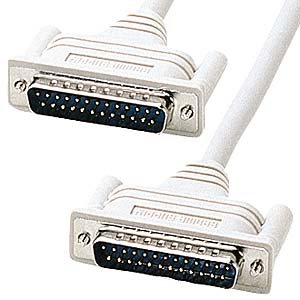
\includegraphics[width=0.35\textwidth]{./img/rs232C}
\caption{RS232C. \cite{RS232C}}
%source:http://image.rakuten.co.jp/menet/cabinet/k_02/krs10107k_ma.jpg?_ex=60x60
\label{fig:RS232C}}
\qquad
\begin{minipage}{5cm}
\centering
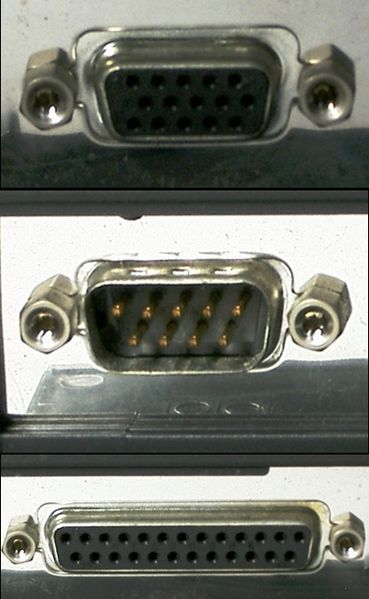
\includegraphics[width=0.7\textwidth]{./img/rs232family}
\caption{Rodzina RS232. \cite{RS232family}}
%source:https://upload.wikimedia.org/wikipedia/commons/thumb/2/20/VGA-RS-232C-Parallelbus.jpg/369px-VGA-RS-232C-Parallelbus.jpg
\label{fig:RS232Family}
\end{minipage}
\end{figure}
\noindent Złącza typu RS232C można jeszcze spotkać jako interfejs komunikacyjny z drukarkami starego typu, niemniej został on wyparty przez nowsze interfejsy (takie jak np. USB). \\
\indent Interfejsami najbardziej wydajnymi są USB oraz Ethernet. Są to stosunkowo nowo opracowane (w porównaniu do RS232) i nadal rozwijane interfejsy. Dokładny opis standardu USB znajduje się w rozdziale \ref{USBStandardChapter}.
Warto również wspomnieć, że najtrudniejszym do zaimplementowania protokołem/interfejsem przesyłania danych jest Bluetooth (w wypadku kategoryzacji według takiego wyznacznika). Służy on do bezprzewodowej komunikacji na bardzo krótkim dystansie.
\newline
\indent Podsumowując, interfejsy szeregowe umożliwiają komunikację miedzy urządzeniami, z których jeden najczęściej jest komputerem osobistym. Implementacja każdego interfejsu jest na swój sposób złożona. Kategoryzacja jest możliwa na podstawie różnych wielkości. W tym rozdziale zostały podzielone według złożoności interfejsu (w sensie architektury), wydajności oraz trudności implementacji.

\section{Opis USB}
\label{USBStandardChapter}
Uniwersalna Magistrala Szeregowa jest to standard opracowany w latach 90. XX w. definiujący jakie kable, złącza oraz protokoły mają być używane podczas połączenia, komunikacji oraz definiuje sposób zasilania pomiędzy komputerem i urządzeniem elektronicznym. USB zostało zaprojektowane aby ułatwić połączenia standardowych elektronicznych urządzeń takich jak klawiatury, myszki, drukarki, aparaty cyfrowe, dyski przenośne do komputerów osobistych. Wszystkie te urządzenia są dodatkowo zasilane również za pomocą tego portu. Z czasem stało się to wspólne również dla innych urządzeń takich jak smartphony, palmtopy oraz konsole wideo.\cite{USBSystemArch, USB20Doc, USB30Doc}
\newline
\indent USB szybko zastąpiło porty szeregowe oraz równoległe podobnie jak inne urządzenia będące źródłem zasilania dla innych układów scalonych. Istnieją trzy podstawowe rodzaje złączy USB, dla których kryterium podziału stanowi wielkość (wtyczki). Najstarszy rozmiar (używany np. w pendrive'ach - typ A) występuje w standardach USB1.1, USB2.0, USB3.0, mini-USB (początkowo tylko dla złącza typu B, jak w wypadku wielu aparatów cyfrowych) oraz mikro-USB występuje również w trzech wariantach dla USB1.1, USB2.0, USB3.0 (dla przykładu używany w nowych telefonach komórkowych). 
\newline
\indent W przeciwieństwie do innych kabli do przesyłu danych (np. Ethernet, HDMI) każdy koniec kabla zakończony jest innym typem złącza (typem A lub typem B). Tylko złącze typu A jest odpowiedzialne za dostarczenie zasilania do złącza typu B. Zostało ono zaprojektowane w taki sposób aby uniknąć elektrycznych przeciążeń, a co za tym idzie uszkodzeniu urządzenia. Istnieją również kable ze złączami typu A na obu końcach, ale nie należą do popularnych (i należy postępować z nimi ostrożnie). Kable USB maja zazwyczaj złącze typu A (męskie) z jednej strony oraz złącze typu B z drugiej (również męskie) oraz wejście w komputerze lub urządzeniu elektronicznym (żeńskie). W przyjętej praktyce złącze typu A jest zazwyczaj największej (z możliwych) wielkości, natomiast B w zależności od potrzeb użycia kabla (full, mini, micro). \cite{USBSystemArch, USB20Doc, USB30Doc, DevUSBPher}

\begin{figure}[h]
\centering

\includegraphics[width=0.5\textwidth]{./img/usbLogo}
\caption{Logo standardu USB2.0 oraz USB3.0. \cite{usbLogo}}
\end{figure}
%
% USB ON THE GO ??
%
%%\section{Historia}
\indent USB zapoczątkowało w 1994 siedem firm: Compaq, DEC, IBM, Intel, Microsoft, NEC, Nortel. Celem było uproszczenie podłączenia zewnętrznych urządzeń do komputera zastępując stare złącza w płytach głównych wprowadzając rozwiązania na problemy znalezione w starych oraz upraszczając software.
Pierwszy układ scalony wspierający USB został wyprodukowany przez Intel 1995r.
\newline
%%\subsection{USB1.x}
\indent Pierwsza oficjalna wersja standardu USB została wydana w styczniu 1996r. USB1.0 charakteryzowała prędkość 1,5 Mbit/s (Low Speed) oraz 12 Mbit/s (Full Speed). Nie pozwalał jednak na używanie przedłużaczy kabli, wynikało to z limitów zasilania. %todo: to zdanie nie ma sensu 
Kilka powstałych wypuszczono na rynek na chwile przed wydaniem standardu USB1.1 w sierpniu 1998r. W USB1.1 poprawiono kilka błędów znalezionych w USB1.0 i był to pierwszy standard, który został oficjalnie zaimplementowany w standardowych komputerach osobistych. \cite{USBSystemArch}
%%\subsection{USB2.0}
\newline
\indent USB2.0 zostało wydane w kwietniu 2000r. udostępniając maksymalny przesył sygnału rzędu 480 Mbit/s (60MB/s) nazwany High Speed (USB1.x za pomocą Full Speed umożliwiał przesył rzędu 12Mbit/s). Biorąc pod uwagę zależności dostępu do magistrali przepustowość High Speed ogranicza się do 280 Mbit/s (35 MB/s).
Przyszłe modyfikacje do specyfikacji USB zostały zaimplementowane przez "Engineering Change Notitices" (ECN). Najważniejsze z ECNów zostały dołączone do specyfikacji USB2.0, dostępnej na stronie internetowej USB.org.
Przykłady ECNow to
Złącze Mini-A oraz Mini-B: wydane w październiku 2000r.\cite{USB20Doc}
\newline
%%\subsection{USB3.0}
\indent Standard USB3.0 został wydany w listopadzie 2008r. definiując zupełnie nowy tryb "SuperSpeed". Port USB zwyczajowo jest w kolorze niebieskim i jest on kompatybilny z urządzeniami USB2.0 oraz kablami.
Dokładnie 17 listopada 2008r. ogłoszono iż specyfikacja dla wersji 3.0 została całkowicie ukończona i została zaakceptowana przez "USB Implementers Forum" (USB-IF), czyli głównej instytucji zajmującej się specyfikacjami standardu USB. To pozwoliło na szybkie udostępnienie standardu deweloperom.
Nowa magistrala "SuperSpeed" dostarcza czwarty typ transferu z możliwością przesyłania sygnału z prędkością 5GBit/s, ale poprzez użycie kodowania 8b/10b przepustowość wynosi 4Gbit/s. Specyfikacja uznaje za zasadne osiągniecie prędkości w okolicach 3,2 Gbit/s (400 MB/s), co w założeniach powinno się zwiększać wraz z rozwijaniem hardwaru. Komunikacja dla SuperSpeed odbywa się w obu kierunkach (kierunek nie jest naprzemienny i nie jest kontrolowany przez hosta, jak to ma miejsce do wersji USB2.0).
Podobnie jak w poprzednich wersjach standardu, porty USB3.0 działają dwóch wariantach zasilania: niskiego poboru mocy (low-power: 150mA) oraz wysokiego poboru mocy (high-power: 900mA). Zapewniając odpowiedni, jednocześnie pozwalają na przesył danych z prędkością SuperSpeed.
Została dodatkowo zdefiniowana specyfikacja zasilania (w wersji 1.2 wydana w w grudniu 2010r.), która zwiększała dopuszczalny pobór mocy do 1,5A, ale nie pozwala na współbieżne przesyłanie danych. Specyfikacja wymaga aby fizyczne porty same w sobie były w stanie obsłużyć 5A, ale ogranicza pobór do 1,5 A.
\cite{USB30Doc}
\newline
%\subsection{USB3.1}
\indent W styczniu 2013r. w prasie pojawiły się informacje o planach udoskonalenia standardu USB3.0 do 10Gbit/s. Zakończyło się to stworzeniem nowej wersji standardu - USB3.1. Wersja ta została wydana 31 lipca 2013r. wprowadzając szybszy typ przesyłania danych zwany "SuperSpeed USB 10 Gbit/s". Zaprezentowano również nowe logo stylizowane na zasadzie "Superspeed+". Standard USB3.1 zwiększył szybkość przesyłu sygnału do 10Gbit/s. Udało się też zredukować obciążenie łącza do 3\% dzięki zmianie kodowania na 128b/132b.
Przy pierwszych testach prędkości USB3.1 udało się uzyskać wynik na poziomie 7,2Gbit/s. Standard USB3.1 jest wstecznie kompatybilny ze standardem USB3.0 oraz USB2.0.
\cite{USB30Doc}
\newline
\indent Poszczególne rodzaje kodowania dla standardów USB3.0 oraz USB3.1 to kodowanie 8bitów na 10 bitów oraz 128 bitów na 132 bity. 
Jeśli chodzi o przesyłanie danych to do momentu wprowadzenia Differential signaling (polega na wysłaniu dwóch przeciwnych sobie sygnałów TX+ oraz TX- do zewnętrznego odbiornika, który aby zniwelować zaszumienie odejmuje wartość RX- od obydwu kanałów) przesyłanie danych na długie odległości lub wysyłanie danych z większą prędkością było awykonalne. Przykład wraz z kolejnymi etapami widoczny na rys \ref{fig:cleanSignal}, \ref{fig:receivedNoiseSignal}, \ref{fig:receivedCleanedSignal}.
\newline
\indent W czasach kiedy elektronika miała swoje początki, zarówno nadawca jak i odbiorca współdzielili to samo uziemienie (były częścią jednego środowiska), więc nie było problemów aby zmierzyć napięcie sygnału wejściowego. Więc jeżeli założenie było iż 0V reprezentuje wartość bitu równą '0' a wartość +5V reprezentuje wartość bitu równą '1' oraz zegar był również wspólny dla nadajnika oraz odbiorcy, odbiorca świetnie potrafił odczytać nadawany sygnał (np. rys. \ref{fig:cleanSignal}).
\begin{figure}[H]
\centering
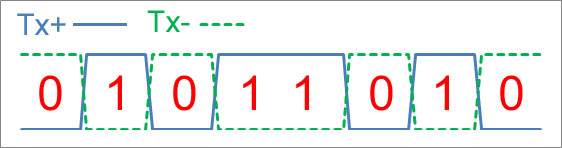
\includegraphics[width=0.7\textwidth]{./img/cleanSignal}
\caption{Przykład czystego (bez zakłóceń) sygnału transmitowanego. \cite{cleanSignal}}
%source: http://eecatalog.com/usb/files/2012/06/120606_lecroy_1.jpg
\label{fig:cleanSignal}
\end{figure}
\noindent Problem pojawia się w momencie kiedy odbiornik znajduje się poza środowiskiem nadawcy (nadawca i odbiorca nie współdzielą uziemienia, zegara, etc.). Rys. \ref{fig:receivedNoiseSignal} przedstawia sygnał odebrany po stronie odbiornika (jest to ten sam sygnał co na rys. \ref{fig:cleanSignal}). Przez brak współdzielenia uziemienia oraz zegara przez nadajnik oraz odbiornik sygnał stał się nieczytelny po stronie odbiornika.
\begin{figure}[H]
\centering
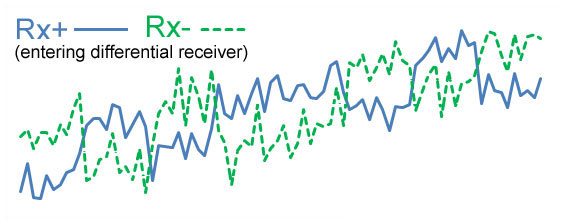
\includegraphics[width=0.7\textwidth]{./img/receivedNoiseSignal}
\caption{Przykład odebranego sygnału (wraz z zakłóceniami). \cite{receivedNoiseSignal}}

%source: http://eecatalog.com/usb/files/2012/06/120606_lecroy_2.jpg
\label{fig:receivedNoiseSignal}
\end{figure}
\begin{figure}[H]
\centering
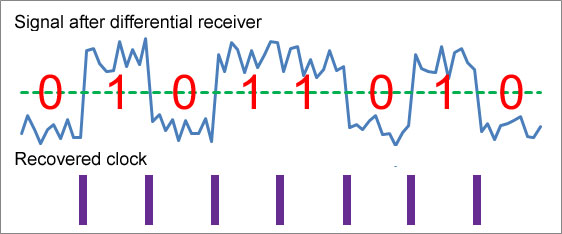
\includegraphics[width=0.9\textwidth]{./img/receivedCleanedSignal}
\caption{Przykład sygnału po oczyszczeniu z szumów. \cite{receivedCleanedSignal}}
%source: http://eecatalog.com/usb/files/2012/06/120606_lecroy_3.jpg
\label{fig:receivedCleanedSignal}
\end{figure}
\noindent Rozwiązaniem problemu przesyłu danych między dwoma zewnętrznymi elektronicznymi urządzeniami okazało się zaprojektowanie differential receiver'a, czyli odbiornika odbierającego dwa sygnały RX+ oraz RX-. Poziom sygnału jest mierzony na podstawie ich złożenia. Skrętka\footnote{Skrętka - w kontekście pary skręconych przewodów} gwarantuje, że przesunięcie napięcia (rys. \ref{fig:receivedNoiseSignal}) dla obu kanałów jest takie samo, a więc różnica pomiędzy jest stała i jest możliwa do odczytu przez odbiornik (rys. \ref{fig:receivedCleanedSignal}). Dodatkowo odbiornik jest w stanie odczytać sygnał zegara na podstawie szybkości zmian sygnału (rys. \ref{fig:receivedCleanedSignal}).
\newline
\indent W przypadku wysyłania większej ilości danych pojawia się kolejny problem. Jeżeli ilość tych samych wartości bitu (zer lub jedynek) występujących po sobie jest zbyt duża, odbiornik może nie być w stanie odczytać sygnału zegara lub zrobić to błędnie. Rys. \ref{fig:withoutEncoding} zawiera przykładowy zestaw wysyłania większej ilości zer, jak widzimy, w drugim i trzecim pakiecie danych wysyłane są same zera, a ilość przeskoków sygnału (zmian 0->1 lub 1->0) jest znikoma i obliczenie sygnału zegara może być problematyczne dla odbiornika.

\begin{figure}[H]
\centering
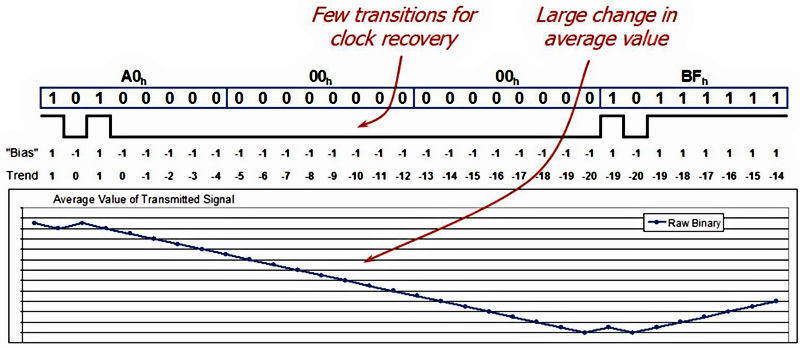
\includegraphics[width=0.95\textwidth]{./img/withoutEncoding}
\caption{Przykład sekwencji danych bez kodowania. \cite{withoutEncoding}}
%source: http://m.eet.com/media/1158450/tek8b-10bfig1.jpg
\label{fig:withoutEncoding}
\end{figure}
\noindent Rozwiązaniem tego problemu jest kodowanie 8b/10b, dzięki któremu ilość zmian sygnału z zera na jeden oscyluje w okolicach 50\% w stosunku do zmian z jeden na zero, dzięki czemu obliczenie zegara na odbiorniku nie jest problematyczne. Przykład sygnału po zastosowaniu kodowania 8b/10b jest widoczny na rys. \ref{fig:withEncoding}.
\begin{figure}[H]
\centering
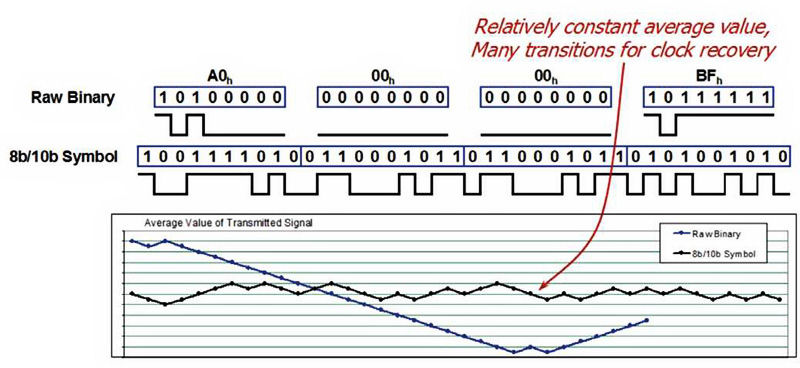
\includegraphics[width=0.8\textwidth]{./img/withEncoding}
\caption{Przykład sekwencji po zakodowaniu. \cite{withEncoding}}
%http://m.eet.com/media/1158451/tek8b-10bfig2.jpg
\label{fig:withEncoding}
\end{figure}
Rys. \ref{fig:sendingDataThroughPHYLayer} przedstawia działanie USB3.0 wraz z kodowaniem oraz komunikacją przez warstwę fizyczną. Najpierw dane do wysłania przekonwertowywane są na z postaci 8-bitowej na postać 10-bitową, następnie wysyłane do odbiornika, gdzie następuje konwersja odwrotna do postaci 8-bitowej.
\begin{figure}[H]
\centering
\includegraphics[width=0.9\textwidth]{./img/SendingData}
\caption{Przykład wysyłania danych przez warstwę fizyczną wykorzystując kodowanie. \cite{SendingData}}
%source: http://eecatalog.com/usb/files/2012/06/120606_lecroy_4.jpg
\label{fig:sendingDataThroughPHYLayer}
\end{figure}
\indent Kodowanie 8b/10b w swojej budowie jest kombinacją dwóch innych: 5b/6b oraz 3b/4b z zachowaniem odpowiedniej zasady ich łączenia. Cały algorytm tworzenia przedstawia się następująco:
\begin{enumerate}
\item 8 bitów jako dane wejściowe: HGFEDCBA\footnote{HGFEDCBA - liczba zapisana binarnie w postaci 8 bitów, gdzie H jest najbardziej znaczącym bitem a A jest najmniej znaczącym bitem},
\item na ostatnich 5 bitach (EDCBA) wykonujemy kodowanie 5b/6b (dochodzi dodatkowy bit),
\item na pierwszych trzech bitach (HGF) wykonujemy kodowanie 3b/4b (dochodzi kolejny bit),
\item całość łączona do postaci abcdeifghj\footnote{abcdifhgj - 10 bitowy rezultat kodowania 8b/10b, należy zwrócić uwagę iż kolejność najbardziej znaczącego i najmniej znaczącego bitu jest odwrócona w stosunku do danych wejściowych, oraz i, j, są dodatkowymi dwoma bitami} tworząc rezultat (przedstawiony na rys. \ref{fig:810mapping}).
\end{enumerate}
%Rysunek \ref{fig:810mapping} doskonale przedstawia ten proces.
\begin{figure}[H]
\centering
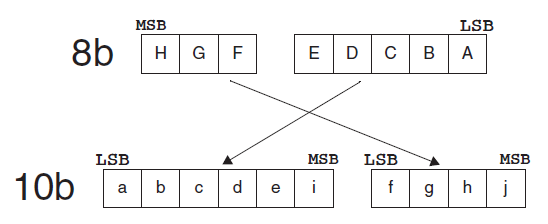
\includegraphics[width=0.75\textwidth]{./img/mapping810}
\caption{Przykład mapowania w kodowaniu 8b/10b. \cite{mapping810}}
%http://m.eet.com/media/1158451/tek8b-10bfig2.jpg
\label{fig:810mapping}
\end{figure}

Dwa ostatnie bity ustala się oddzielnie dla tych dwóch kodowań, na podstawie współczynnika RD\footnote{RD (ang. Running Disparity) - różnica pomiędzy ilością jedynek i zer w ciągu)}, czyli różnicy pomiędzy ilością jedynek i zer w ciągu. Jak zostało wspomniane wyżej, założenie całego kodowania jest takie aby, ilość zer całości przesyłanych danych oscylowała w okolicach 50\%, więc różnica (RD) dla jednego zestawu 10 bitów danych wynosi +-2.
\newline
\indent Realizacja kodowania 5b/6b jest nieco bardziej skomplikowana, polega bowiem na takim dopasowaniu '0' i '1' aby różnica pomiędzy ich ilością była równa +-1 (jest to tak na prawdę RD lub odległość Hamminga\footnote{odległość Hamminga - w kontekście projektu XOR dwóch zbiorów}). Wartość wyjściowa musi być unikalna. Jest to możliwe dzięki dodaniu do zbioru dodatkowego bitu (unikalność mogłaby zostać zachowana bez niego, natomiast nie zostałby spełniony warunek RD = +-1).
\newline
\iffalse 
%Todo: na razie wylaczone
%\begin{tabular}{ | a | l | l | l | a | l | l | l | }
\begin{table}[H]
\begin{tabular}{|>{\columncolor[gray]{0.85}}c|c|c|c|>{\columncolor[gray]{0.85}}c|c|c|c|c|}
\cline{1-9}
	\rowcolor[gray]{0.7}
	 & \mc{1}{} & \mc{1}{RD = -1} & RD = +1 &  & \mc{1}{} & \mc{1}{RD = -1} & RD = +1 \\ \cline{1-9}
	\rowcolor[gray]{0.75}
	 & \mc{1}{EDCBA} & \mc{1}{abcdei} & abcdei &  &  \mc{1}{EDCBA} & \mc{1}{abcdei} & abcdei \\ \hline
	D.00 & 00000 & 100111 & 011000 &  D.16 & 10000 & 011011 & 100100 \\ \hline
	D.01 & 00001 & 011101 & 100010 &  D.17 & 10001 & \mc{1}{100011} &  \\ \hline
	D.02 & 00010 & 101101 & 010010 &   D.18 & 10010 & \mc{1}{010011} &  \\ \hline
	D.03 & 00011 & \mc{1}{110001} &  &  D.19 & 10011 & \mc{1}{110010} &  \\ \hline
	D.04 & 00100 & 110101 & 001010 &   D.20 & 10100 & \mc{1}{001011} &  \\ \hline
	D.05 & 00101 & \mc{1}{101001} &   & D.21 & 10101 & \mc{1}{101010} &  \\ \hline
	D.06 & 00110 & \mc{1}{011001} &    & D.22 & 10110 & \mc{1}{011010} &  \\ \hline
	D.07 & 00111 & 111000 & 000111 &   D.23& 10111 & 111010 & 000101 \\ \hline
	D.08 & 01000 & 111001 & 000110 &   D.24 & 11000 & 110011 & 001100 \\ \hline
	D.09 & 01001 & \mc{1}{100101} &    & D.25 & 11001 & \mc{1}{100110} &  \\ \hline
	D.10 & 01010 & \mc{1}{010101} &  & D.26 & 11010 & \mc{1}{010110} &  \\ \hline
	D.11 & 01011 & \mc{1}{110100} &    & D.27 & 11011 & 110110 & 001001 \\ \hline
	D.12 & 01100 & \mc{1}{001101} &    & D.28 & 11100 & \mc{1}{001110} &  \\ \hline
	D.13 & 01101 & \mc{1}{101100} &    & D.29 & 11101 & 101110 & 010001 \\ \hline
	D.14 & 01110 & \mc{1}{011100} &   & D.30 & 11110 & 011110 & 100001 \\ \hline
	D.15 & 01111 & 010111 & 101000 &   D.31 & 11111 & 101011 & 010100 \\ \hline
	 &  &  &  &   K.28 & 11100 & 001111 & 110000 \\ \hline
\end{tabular}
\captionof{table}{Przykład mapowania 5b na 6b \cite{tablesMapping}}
%source: 
\label{tbl:5bTo6b}
\end{table}


\begin{table}[H]

%\begin{tabular}{ | l | l | l | l | l | l | l | l | }
\begin{tabular}{|>{\columncolor[gray]{0.85}}c|c|c|c|>{\columncolor[gray]{0.85}}c|c|c|c|c|}
\hline
\cline{1-9}
	\rowcolor[gray]{0.7}
	 &  & \mc{1}{RD = -1} & \mc{1}{RD = +1} & \mc{1}{} & \mc{1}{} & \mc{1}{RD = -1} & RD = +1 \\ 
	\cline{1-9}
	\rowcolor[gray]{0.75}
	 & \mc{1}{HGF} & \mc{1}{fghj} & \mc{1}{fghj} &  & \mc{1}{HGF} & \mc{1}{fghj} & fghj \\ \hline
	D.x.0 & 000 & 1011 & 0100 & K.x.0 & 000 & 1011 & 0100 \\ \hline
	D.x.1 & 001 & \mc{1}{1001} &  & K.x.1 & 001 & 0110 & 1001 \\ \hline
	D.x.2 & 010 & \mc{1}{0101} &  & K.x.2 & 010 & 1010 & 0101 \\ \hline
	D.x.3 & 011 & 1100 & 0011 & K.x.3 & 011 & 1100 & 0011 \\ \hline
	D.x.4 & 100 & 1101 & 0010 & K.x.4 & 100 & 1101 & 0010 \\ \hline
	D.x.5 & 101 & \mc{1}{1010} &  & K.x.5 & 101 & 0101 & 1010 \\ \hline
	D.x.6 & 110 & \mc{1}{0110} &  & K.x.6 & 110 & 1001 & 0110 \\ \hline
	D.x.P7 & 111 & 1110 & 0001 &  &  &  &  \\ \hline
	D.x.A7 & 111 & 0111 & 1000 & K.x.7 & 111 & 0111 & 1000 \\ \hline
\end{tabular}
\captionof{table}{Przykład mapowania 3b na 4b \cite{tablesMapping}}
%source: 
\label{tbl:3bTo4b}
\end{table}
\fi
%\newline
\noindent Sporą część kodów da się wyliczyć na podstawie zamiany EDCBA -> abcfe (odwrócenie bitów) oraz dodanie wartości '0' lub '1' w zależności od aktualnej wartości RD. Niestety nie dotyczy to wszystkich elementów. Istnieją 32 wartości wraz z przekonwertowanymi odpowiednikami oraz jedna konwersja dla instrukcji kontrolnej.
%todo later today
\newline
\noindent Konwersja 3b/4b zawiera dwie specyficzne (podkonwersje): podstawową (ang. primary) oraz alternatywną (ang. alternative). Dodatkowa alternatywna konfiguracja dla tego zestawu danych została stworzona w celu uniknięcia 5-elementowego ciągu złożonego z samych zer lub jedynek podczas łączenia z kodowaniem 5b/6b, czyli tworzeniem kodu 8b/10b (a w wypadku samego podstawowego zestawu byłoby to o wiele trudniejsze).
\newline
\noindent Tabela \ref{tbl:controllchars} przedstawia instrukcje kontrolne w postaci zakodowanej w zależności od Running Disparity (RD). Jest to doskonały przykład jak wyglądają tego typu kody. 
\begin{table}[H]
%\begin{tabular}{ | l | l | l | l | l | l | }
\centering
\begin{tabular}{|>{\columncolor[gray]{0.85}}c|c|c|c|c|c|}
\hline

	\rowcolor[gray]{0.7}
	\mc{1}{} & \mc{1}{} &  &  & RD = -1 & RD = +1 \\ \hline
	\rowcolor[gray]{0.75}
	 & \mc{1}{DEC} & HEX & HGF EDCBA & abcdei fghj & abcdei fghj \\ \hline
	K.28.0 & 28 & 1C & 000 11100 & "001111 0100 & "110000 1011 \\ \hline
	K.28.1 & 60 & 3C & "001 11100" & "001111 1001 & "110000 0110 \\ \hline
	K.28.2  & 92 & 5C & "010 11100 & "001111 0101 & "110000 1010 \\ \hline
	K.28.3  & 124 & 7C & "011 11100 & "001111 0011 & "110000 1100 \\ \hline
	K.28.4  & 156 & 9C & "100 11100 & "001111 0010 & "110000 1101 \\ \hline
	K.28.5  & 188 & BC & "101 11100 & "001111 1010 & "110000 0101 \\ \hline
	K.28.6  & 220 & DC & "110 11100 & "001111 0110 & "110000 1001 \\ \hline
	K.28.7  & 252 & FC & "111 11100 & "001111 1000 & "110000 0111 \\ \hline
	K.23.7  & 247 & F7 & "111 10111 & "111010 1000 & "000101 0111 \\ \hline
	K.27.7  & 251 & FB & "111 11011 & "110110 1000 & "001001 0111 \\ \hline
	K.29.7  & 253 & FD & "111 11101 & "101110 1000 & "010001 0111 \\ \hline
	K.30.7  & 254 & FE & "111 11110 & "011110 1000 & "100001 0111 \\ \hline
\end{tabular}
\captionof{table}{Przykład komunikatów kontrolnych \cite{tablesMapping}}
%source: 
\label{tbl:controllchars}
\end{table}
\indent Kodowane zaimplementowane w standardzie USB3.1 (128b/132b) różni się nieco od swojego poprzednika. W kodowaniu 128b/132b pierwsze cztery bity zostały przeznaczone na header, a pozostałe 128 bitów na dane. W porównaniu do kodowania 8b/10b, gdzie mieliśmy tak naprawdę utratę 20\% możliwości łącza, przez reprezentację każdej porcji 8 bitów - 10 bitowym kodem, to wartość ta spada do 3\%. Dodatkowo dzięki pierwszym czterem bitom możliwe jest określenie czy przesyłane są dane do przetworzenia czy wysyłane jest polecenie kontrolne. Dane są obudowywane w pakiety o znanym rozmiarze (zawartym w headerze) o maksymalnej wartości równej 128 bity.
\begin{figure}[H]
\centering
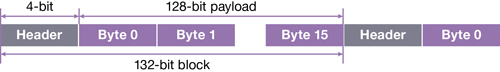
\includegraphics[width=0.9\textwidth]{./img/128to132coding}
\caption{Schemat ramki w kodowaniu 128b/132b. \cite{128to132coding}}
%source: http://www.synopsys.com/Company/Publications/DWTB/PublishingImages/dwtb-q4/dwtb-q414-usb3-fig1.jpg
\label{fig:128to132coding}
\end{figure}
\indent Sterowniki dla najczęściej używanych urządzeń USB (np. pendrive) instalują się automatycznie na dzisiejszych systemach operacyjnych (ponieważ system operacyjny posiada informacje na temat urządzeń najczęściej użytkowanych), ma to miejsce zaraz po podłączeniu urządzenia do wejścia USB w komputerze osobistym (mechanizm plug-and-play). Celem takiego rozwiązania było jak największe ułatwienie użytkownikowi dostępu do najbardziej spopularyzowanych urządzeń (najczęściej nośników danych, kamer internetowych, etc..). Założeniem projektu było napisanie aplikacji która wymienia dane z urządzeniem niestandardowym (dedykowanym do bardziej złożonych zadań), a co za tym idzie system operacyjny nie był w posiadaniu odpowiednich sterowników dla urządzenia testowego (dokładnie opisanego w rozdziale \ref{microcontrollerChapter}). Ten sam przypadek będzie miał miejsce z wykorzystaniem innego urządzenia do testów, lub też, w wypadku wykorzystania komercyjnego, należy zadbać o odpowiednią instalację sterownika. Jeśli chodzi o systemy z rodziny UNIX należy zainstalować bibliotekę (opisaną w rozdziale \ref{libUsbChapter}) używając typowego mechanizmu dla systemów UNIXowych\footnote{w wypadku Ubuntu jest to komenda "sudo apt-get install libusb-1.0-0-dev", gdzie libusb-1.0-0-dev jest nazwą pakietu, zawierającego wszystkie potrzebne elementy biblioteki opisanej w późniejszych rozdziałach}. Jest to jedyna czynność jaką należy wykonać przed rozpoczęciem pracy nad implementacją. W przypadku produktów Microsoftu, sprawa przedstawia się nieco inaczej. Wymagana jest instalacja sterownika, który pozwala systemowi na identyfikacje urządzenia. Istotna tutaj jest instalacja sterownika dla każdego nieznanego (nowo podłączonego) przez system urządzenia oddzielne, a dokładniej przy pierwszym użyciu (systemy z rodziny Windows rozpoznają urządzenia połączone interfejsem USB po ich znanej wcześniej VendorId oraz ProductId\footnote{VendorId, ProductId - id specyficzne dla każdego urządzenia, opisane w dalszych rozdziałach}, stad instalacja sterownika odwołuje się do konkretnego podłączonego urządzenia). Po spełnieniu powyższych wymagań możliwe jest pełne wykorzystanie możliwości bibliotek.
\newline
\indent Podsumowując, USB należy do rozbudowanych interfejsów poprzez wieloletnie udoskonalanie produktu oraz dążenie do poprawy szybkości przesyłu danych. Dzięki pracy wielu inżynierów oraz udoskonalaniu kodowania znaków, aby rozwiązywać coraz to nowo napotykane problemy, jest to najbardziej powszechny interfejs udostępniony do użytku publicznego. System operacyjny zapewnia szybką instalację sterowników dla podstawowych (najczęściej spotykanych dla użytku domowego) urządzeń. W wypadku bardziej rozbudowanych to programista ma za zadanie zadbać o odpowiednie sterowniki.
\section{Testy jednostkowe, komponentowe, automatyczne i wydajnościowe}
\indent Tworzenie testów jest nieodłączną częścią tworzenia oprogramowania. Istnieje wiele metodologi stosowanych w tym temacie, a do najbardziej popularnych należy TDD\footnote{TDD - ang. Test Driven Development} polegająca na stworzeniu przez programistę/testera testu na podstawie wymagań danej funkcjonalności, zanim powstanie do niego implementacja właściwa. Metodologia ta ma swoje plusy jak i minusy. Plusem z pewnością jest weryfikacja funkcjonalności w trakcie pisania kodu produktu (widoczny jest postęp, choć sam w sobie test jeszcze nie przechodzi). Po zakończeniu funkcjonalności możliwy jest pożądany refaktoring kodu, mający na celu zwiększenie przejrzystości dla osób rozwijających projekt dalej. Dzięki zaimplementowanym wcześniej testom istnieje możliwość wstecznego sprawdzania funkcjonalności, innymi słowy czy refaktoring zbytnio nie uszkodził funkcjonalności stworzonego kodu.
\newline
\indent Testy dzielą się na kilka grup ze względu na ich funkcjonalność. Podstawowym rodzajem są testy jednostkowe (UT\footnote{UT - Unit Tests}) polegające na testowaniu zachowania poszczególnej funkcji czy też metody. Internet szerzy się od różnego rodzaju frameworków dla UT. Do jednych z najpopularniejszych należy Google Test (jeśli chodzi o C++), który posiada bardzo łatwy do nauczenia się i przystępny framework. Za ich pomocą można testować wynik wyjściowy poszczególnych metod/funkcji, jak również sprawdzać działanie jeśli za argumenty przyjmują wskaźniki. Istnieje również możliwość łatwego zbadania co dana metoda zrobiła z danym obiektem (którego wskaźnik został podany jako argument).
\newline
\indent Kolejnym rodzajem testów jakie powinny być przeprowadzane w miarę możliwości są testy komponentowe (SCT\footnote{SCT - Software Component Tests}). W tym wypadku testowanie odbywa się na zupełnie innych zasadach i nie zawsze jest aplikowalne do każdego projektu. Testy komponentowe należy tworzyć jeżeli projekt/produkt zawiera w sobie więcej niż jeden komponent\footnote{tutaj w rozumieniu procesu} oraz istnieje zaprojektowana interakcja na interfejsach zdefiniowanych miedzy nimi. Innymi słowy warunkiem koniecznym jest aby te dwa (lub więcej) komponenty komunikowały się ze sobą za pomocą wiadomości. Istotą komponent testów jest to, iż przygotowuje się zbliżone środowisko do docelowego (jeżeli aplikacja działa na hardwarze o określonej architekturze katalogów to należy dostarczyć zbliżoną architekturę do docelowej, często stosuje się do tego kontenery), a następnie uruchamia się tylko i wyłącznie testowany komponent, a jego otoczenie (inne procesy komunikujące się z nim w projekcie) symuluje. Cały test polega na bombardowaniu testowanego komponentu wiadomościami aby wymusić odpowiednie zachowanie. Dla przykładu istnieją 3 komponenty A, B oraz C, testowanym jest komponent B, wiadomo, że w docelowym zachowaniu komponent A wysyła do komponentu B wiadomość x, a komponent B po wykonaniu kilku operacji wysyła wiadomość y do komponentu C. Programista testując komponent B powinien mu wstrzyknąć wiadomość x (której struktura w teście jest znana) za pomocą symulowanego komponentu A i sprawdzić czy w takim przypadku symulowany komponent C otrzyma wiadomość y. Jeśli tak się niestanie oznacza to, że jeszcze jakaś część komponentu B nie została zaimplementowana według wymagań, w przeciwnym wypadku test uznał pewną zależność komponentów za poprawną. Popularnymi językami w których istnieje możliwość pisania testów komponentowych są Python oraz ttcn3.
\newline
\indent Istnieje również automatyzacja testów. Stosuje się ją w wypadku większych zmian aby mieć pewność iż wprowadzanie nowych funkcjonalności nie naruszyło poprzednich. Automatyzuje się przede wszystkim testy weryfikacyjne (SyVe\footnote{SyVe - System Verification}), które w standardowym (albo w większości procesów) polegają na manualnym testowaniu danych funkcjonalności i weryfikowaniu czy otrzymany został pożądany rezultat. Istotną rolę pełnią również testy integracyjne aplikowalne tylko do większych projektów, w których istotną role odgrywa współdziałanie wielu komponentów, z reguły implementowane przez różne zespoły.
\newline
\indent Z punktu widzenia pracy najbardziej istotna jest weryfikacja oprogramowania z początkowymi założeniami (wymaganiami). Należy zadbać o powtarzalność testu i o przejrzystość formatu danych wyjściowych. Testy należy wykonać w środowisku docelowym (z zewnętrznym urządzeniem) aby uniknąć późniejszych wątpliwości. Należy również przygotować środowisko dla automatyzacji. Testy wykonywane są na specyficznym hardwarze, dokładny opis znajduje się w rozdziale \ref{microcontrollerChapter}.

\chapter{Biblioteki udostępniające API do komunikacji z USB}
\label{librariesChapter}
Głównym celem projektu jest osiągniecie jak najszybszej prędkości przesyłu danych. Do realizacji celu konieczne jest użycie odpowiedniej biblioteki do komunikacji z interfejsem USB. W rozdziale przedstawiony został krótki opis najbardziej popularnych bibliotek posiadających interfejs komunikacyjny ze złączami USB.
\section{Biblioteka libUSB}
LibUSB \cite{libusbDesc} jest biblioteką stworzoną w 2007 roku. Napisana w języku C  pozwala na prosty i łatwy dostęp do urządzenia USB. Jest w 100\% przeznaczona dla użytku developera. Biblioteka ma za zadanie ułatwić pisanie aplikacji opartych na komunikacji USB z mikrokontrolerem.
Jest ona przenośna, a co za tym idzie dostępna na wiele platform (Linux, OS X, Windows, Android, OpenBSD, etc.) wraz z niezmiennym API.
Nie są wymagane dodatkowe uprawnienia aby komunikacja z urządzeniem przebiegała poprawnie.
Wspiera standardy USB: 
\begin{itemize}
\item USB1.0 
\item USB1.1 
\item USB2.0 
\item USB3.0
\end{itemize}
\noindent Funkcjonalność biblioteki:
\begin{enumerate}
\item wszystkie typy transferu są wspierane (control, bulk, interrupt, isochronous)
\item dwa interfejsy
\begin{enumerate}
\item synchroniczny (prosty)
\item asynchroniczny (bardziej złożony)
\end{enumerate}
\item stosowanie wątków jest bezpieczne
\item lekka biblioteka z prostym API
\item kompatybilna wstecznie (do wersji libUSB-0.1)
\end{enumerate}
\section{Biblioteka winUSB}
Microsoft Windows począwszy od systemu Windows Vista wprowadził nowy zestaw bibliotek umożliwiający developerom korzystnie z portów USB. WinUSB udostępnia proste API, które pozwala aplikacji na bezpośredni dostęp do portów USB. Został stworzony w gruncie rzeczy dla prostych urządzeń obsługiwanych tylko przez jedną aplikację, takich jak urządzenia do odczytu wskaźników pogodowych czy też innych programów, które potrzebują szybkiego i bezpośredniego dostępu do portu. WinUSB udostępnia API aby odblokować developera przy pracy z portami USB z poziomu user-mode. W Windowsie 7 USB Media Transfer Protocol (MTP) używa winUSB zamiast poprzednio stosowanych rozwiązań kernela (krenel mode filter driver).

Media Transfer Protocol jest rozszerzeniem PTP (Picture Transfer Protocol) i jest protokołem pozwalającym na przesyłanie atomowe plików audio oraz wideo z oraz do urządzenia. PTP początkowo został zaprojektowany do ściągania zdjęć, obrazów z aparatów cyfrowych. Przykładową implementacją może być przypadek przesyłania danych bezpośrednio z cyfrowych urządzeń odtwarzających muzykę oraz pliki video z urządzeń pozwalających na ich odtworzenie.

MTP jest częścią frameworku "Windows Media" blisko związanym z odtwarzaczem Windows Media Player. Systemy Windows począwszy od Windows XP SP2 wspierają MTP. Windows XP wymaga Windows Media Player w wersji 10 lub wyższej, późniejsze wersje systemu wspierają już go domyślnie. Microsoft posiada dodatkowo możliwość zainstalowania MTP na wcześniejszych wersjach systemu ręcznie do wersji Microsoft Windows 98.

Twórcy standardu USB ustandaryzowali MTP jako pełnoprawną klasę dla urządzeń USB w maju 2008r.
Od tamtej pory MTP jest oficjalnym rozszerzeniem PTP i współdzieli ten sam kod klasy. \cite{winusbDesc, micrDevAppUSBDev, micrAccUsbDev, micCommWithUsb}
\newline

%%%\section{Wybór}
\indent Podsumowując w projekcie została użyta biblioteka libUSB. Głównym powodem była możliwość kompilacji programów zarówno pod systemami Unix jak i z rodziny Microsoft Windows bez jakichkolwiek (lub znikomych) zmian w kodzie.

\chapter{Interfejs udostępniony przez libUSB}
\label{libUsbChapter}
\indent Zadaniem rozdziału jest opis działania poszczególnych funkcji użytych w projekcie. Jest to konieczne aby przeglądając implementacje projektu być w stanie bezproblemowo zrozumieć działanie poszczególnych części projektu. Rozdział został podzielony na podstawie struktur oraz funkcji, których użycie widoczne jest w implementacji właściwej. \cite{libusbDoc}
\newline
\indent Biblioteka pozwala na łatwy dostęp do poszczególnych funkcjonalności standardów USB. Dzieje się to poprzez udostępnienie API\footnote{API (ang. Application Programming Interface) - interfejs (zazwyczaj zestaw funkcji, struktur) umożliwiający programiście na korzystanie z różnych funkcjonalności biblioteki}, dzięki któremu programista może w pełni wykorzystywać możliwości USB. Poniższy rysunek (Rys. \ref{fig:libUsbSchemaLinux}) przedstawia jak zaprojektowano użycie libUSB pod systemami Linuxowymi. Widać, iż aplikacja użytkownika korzysta tylko i wyłącznie z biblioteki libUSB, natomiast sama biblioteka korzysta ze sterownika UsbFs\footnote{UsbFs (ang. Usb filesystem) - wirtualny system plików dostarczający informacji na temat urządzeń USB (podobnie jak /proc na temat procesów}, dzięki czemu zdobywa informacje na temat urządzeń USB. Kolejnym krokiem jest wykorzystanie UsbCore.c oraz sterownika Host Controller. UsbCore.c jest niskopoziomową implementacją standardu USB dla systemów Unixowych, natomiast systemowy sterownik Host Controller pozwala na odblokowanie komunikacji na zewnątrz. To właśnie tutaj zachodzi wydawanie bezpośrednich komend do złącza USB, które jest podłączone bezpośrednio do urządzenia. 
\begin{figure}[H]
\centering
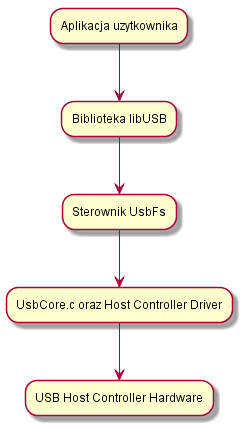
\includegraphics[width=0.35\textwidth]{./img/libUsbSchemaLinux}
\caption{Schemat działania libUSB pod systemami z rodziny Linux.} 
\label{fig:libUsbSchemaLinux}
\end{figure}
\noindent W przypadku działania libUSB dla systemów firmy Microsoft (przedstawione na Rys \ref{fig:libUsbSchemaWindows}) schemat jest nieco uproszczony. Aplikacja korzysta z API udostępnionego przez libUSB (dokładnie z tego samego jak w przypadku działania pod systemem Linux). Natomiast biblioteka libUSB korzysta bezpośrednio ze sterownika zainstalowanego dla konkretnego urządzenia. Pod systemami Windows twórcy biblioteki libUSB stworzyli sterownik, który należy zainstalować oddzielnie dla każdego urządzenia z którym ma przebiegać komunikacja (urządzenie identyfikowane za pomocą vendorId oraz productId - dokładniej opisane w rozdziale \ref{ch:motivationAndBasics}). Poprzez zdanie "za pomocą narzędzi libUSB" (poniższy rys.) rozumiane jest narzędzie pozwalające na łatwą instalacje sterownika dla konkretnego podłączonego urządzenia \cite{zadig}. Sterownik pozwala na komunikacje ze złączem USB.
\begin{figure}[H]
\centering
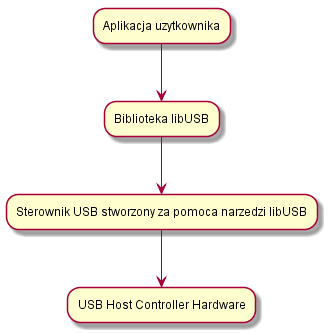
\includegraphics[width=0.55\textwidth]{./img/libUsbSchemaWindows}
\caption{Schemat działania libUSB pod systemami z rodziny Windows.}
\label{fig:libUsbSchemaWindows}
\end{figure}
\noindent Przedstawione powyżej schematy ukazują zasadę działania biblioteki pod poszczególnymi systemami operacyjnymi. W wypadku Linux'a korzysta on z systemowych sterowników, natomiast w wypadku systemu Windows wymagana jest dodatkowa instalacja specyficznego sterownika, który pozwala na przetłumaczenie libUSB API na konkretne działania.

\section{Charakterystyka użytych funkcji}
\subsection{libusb\_init}
\indent Funkcja ta odpowiada za inicjalizację biblioteki.
%\newline
Musi on zostać wywołana przed jakiejkolwiek inną funkcją z biblioteki libUsb.
%\newline
Jeśli w argumencie nie zostanie dostarczony żaden wskaźnik (wyjściowy) kontekstu, zostanie stworzony kontekst domyślny. W przypadku jeśli domyślny kontekst już istnieje zostanie on ponownie użyty (bez inicjalizacji).
%\newline
Funkcja zwraca wartość 0 w wypadku powodzenia, w przeciwnej sytuacji zwraca kod błędu.
\subsection{libusb\_open\_device\_with\_vid\_pid}
\indent Wygodna funkcja służąca do odszukania konkretnego urządzenia na podstawie jego vendorId oraz productId (są to parametry charakteryzujące każde urządzenie).
%\newline
Używana jest w przypadkach kiedy z góry jest znane vendorId oraz productId. Najczęstsze zastosowania znajdują przy pisaniu aplikacji w celu przetestowaniu jakiejś określoną funkcjonalność. Funkcja pozwala uniknąć wywołania libusb\_get\_device\_list() i dbania o odpowiednie czyszczenie pamięci po liście.
%\newline
Pierwszym jej parametrem jest kontekst uzyskany za pomocą libusb\_init().
%\newline
Natomiast kolejnymi parametrami są vendorId oraz productId.
%\newline
Funkcja zwraca uchwyt do znalezionego urządzenia, lub NULL w wypadku kiedy nie może znaleźć pożądanego urządzenia (o podanym productId oraz vendorId) lub błędu.
\subsection{libusb\_kernel\_driver\_active}
\indent Funkcja sprawdzająca czy sterownik jądra kernela jest aktywny na interfejsie.
%\newline
W wypadku kiedy sterownik jądra jest aktywny nie możliwe jest zgłoszenie użycia interfejsu, a co za tym idzie libUSB nie może wykonać operacji wejścia/wyjścia.
%\newline
Funkcjonalność nie jest dostępna w systemie Windows.
%\newline
Do jej zadań należy przekazać uchwyt do urządzenia oraz numer interfejsu.
%\newline
Na wyjściu zwraca ona wartość 0, jeśli żaden sterownik jądra nie jest aktywny, wartość 1 w wypadku jeśli istnieje aktywny sterownik jądra.
\newline
Do zwracanych błędów miedzy innymi należą: LIBUSB\_ERROR\_NO\_DEVICE jeśli urządzenie zostanie odłączone, LIBUSB\_ERROR\_NOT\_SUPPORTED dla platform, gdzie funkcjonalność nie jest wspierana lub gdy występuje inny rodzaj błędu (nie wymieniony wyżej).
\subsection{libusb\_detach\_kernel\_driver}
\indent Dzięki funkcji możliwe jest odłączenie sterownika jądra kernela od interfejsu.
%\newline
Sukces operacji umożliwi zgłoszenie użycia interfejsu i wykonanie operacji wejścia/wyjścia.
%\newline
Funkcjonalność nie jest dostępna dla systemu Windows.
%\newline
Parametrami są uchwyt do urządzenia oraz numer interfejsu.
%\newline
Funkcja zwraca wartość 0 w momencie powodzenia, natomiast w przeciwnym wypadku LIBUSB\_ERROR\_NOT\_FOUND jeśli żaden sterownik nie był aktywny, LIBUSB\_ERROR\_INVALID\_PARAM jeśli interfejs nie istnieje, LIBUSB\_ERROR\_NO\_DEVICE jeśli urządzenie zostało odłączone, LIBUSB\_ERROR\_NOT\_SUPPORTED dla platform, gdzie funkcjonalność nie jest wspierana lub gdy występuje inny rodzaj błędu (nie wymieniony w tej sekcji)
\subsection{libusb\_claim\_interface}
\indent Dzięki funkcji libusb\_claim\_interface() możliwe jest zgłoszenie użycia danego interfejsu dla danego urządzenia.
%\newline
Wywołanie funkcji jest wymagane przed wykonaniem operacji wejścia/wyjścia dla dowolnego punktu końcowego interfejsu.
%\newline
Jest dozwolone wywołanie funkcji dla interfejsu już wcześniej zgłoszonego, w tym wypadku zostanie zwrócona wartość 0 bez wykonywania żadnych operacji.
%\newline
W wypadku jeśli zmienna auto\_detach\_kernel\_driver jest ustawiona na wartość 1 dla danego urządzenia (zmienna ustawiana za pomocą funkcji: libusb\_set\_auto\_detach\_kernel\_driver()) sterownik jądra zostanie odłączony (jeśli to konieczne), w przypadku niepowodzenia zostanie zwrócony błąd odłączenia.
%\newline
Sama procedura wewnątrz funkcji nie jest skomplikowana, nie wymaga wysyłania czegokolwiek po magistrali. Są to proste instrukcje mówiące systemowi operacyjnemu iż aplikacja chce korzystać z danego interfejsu.
%\newline
Nie jest to funkcja blokująca.
%\newline
Parametrami są uchwyt do urządzenia oraz numer interfejsu zgłaszanego.
%\newline
Wartość 0 zostaje zwrócona w wypadku powodzenia operacji.
%\newline
W wypadku niepowodzenia kody błędu t.j. LIBUSB\_ERROR\_NOT\_FOUND jeśli podany interfejs nie istnieje, LIBUSB\_ERROR\_BUSY jeśli inny program lub sterownik zarezerwował dany interfejs, LIBUSB\_ERROR\_NO\_DEVICE jeśli urządzenie zostało odłączone oraz inne.
\subsection{libusb\_bulk\_transfer}
\indent Dzięki funkcji możliwy jest przesył większej grupy danych. Jest to jedna z najważniejszych funkcji użytych w projekcie.
%\newline
Kierunek jest określony na podstawie bitów kierunkowych punktu końcowego interfejsu.
%\newline
Dla odczytu, jeden z parametrów określa ilość danych jaka jest spodziewana przy odczycie. Jeżeli odebrana zostanie mniejsza ilość danych niż oczekiwana, funkcja po prostu zwróci te dane wraz z dodatkowym parametrem określającym ich ilość. Istotne przy odczycie jest to aby sprawdzić, czy ilość oczekiwanych danych jest taka jak odczytana.
%\newline
W wypadku zapisu również należy sprawdzić czy ilość danych wysłanych pokrywa się z ilością danych skierowaną do wysyłki.
%\newline
Wskazana jest również weryfikacja ilości danych wysłanych/odebranych w wypadku wystąpienia timeoutu (funkcja zwróci kod błędu określający timeout). LibUSB może podzielić wysyłane dane na mniejsze części i timeout może wystąpić po wysłaniu kilku z nich. Ważne jest to, że nie oznacza to iż nic nie zostało wysłane/odebrane, dlatego należy sprawdzić ilość elementów wysłanych/odebranych i dostosować odpowiednio kolejne kroki.
%\newline
Funkcja przyjmuje następujące parametry: uchwyt urządzenia z którym aplikacja będzie się komunikować, adres punktu końcowego interfejsu po którym będzie odbywała się komunikacja, wskaźnik do pamięci danych która ma zostać przetransferowana (w wypadku zapisu) lub odebrana (w wypadku odczytu), ilość danych do wysłania (w przypadku zapisu) lub oczekiwana ilość danych do odebrania (w przypadku odczytu), ilość danych przetransferowanych (w obu przypadkach), maksymalna długość czasu na wykonanie operacji, dla nieograniczonego należy użyć wartości równej 0.
%\newline
W przypadku poprawności działania funkcja zwraca wartość 0 oraz ilość przetransferowanych danych przekazanych do funkcji za pomocą wskaźnika.
%\newline
W przeciwnym wypadku funkcja zwraca: LIBUSB\_ERROR\_TIMEOUT jeśli transfer przekroczył określony czas, LIBUSB\_ERROR\_PIPE jeśli wystąpił błąd związany z punktem końcowym, LIBUSB\_ERROR\_OVERFLOW jeśli urządzenie wysłało więcej danych niż przewidziane w buforze, LIBUSB\_ERROR\_NO\_DEVICE jeśli urządzenie zostało odłączone oraz inne.
\subsection{libusb\_release\_interface}
\indent Funkcja zwalnia rezerwacje wcześniej zgłoszonego interfejsu za pomocą funkcji opisanej wyżej (libusb\_claim\_interface).
%\newline
Zwolnienie wszystkich interfejsów jest wymagane przed zamknięciem urządzenia.
%\newline
Nie jest to blokująca funkcja.
%\newline
W wypadku jeśli zmienna auto\_detach\ \newline \_kernel\_driver jest ustawiona na wartość 1 dla danego urządzenia (zmienna ustawiana za pomocą funkcji: libusb\_set\_auto\_detach\_kernel\_driver()) sterownik jądra zostanie ponownie podłączony zaraz po zwolnieniu interfejsu.
%\newline
Parametrami są: uchwyt urządzenia oraz numer interfejsu dla niego poprzednio zarezerwowanego.
\newline
Metoda zwraca 0 gdy wszystkie operacje się powiodą.
%\newline
W przeciwnym wypadku zwraca: LIBUSB\_ERROR\_NOT\_FOUND, jeśli interfejs nie został poprzednio zarezerwowany (zgłoszony do użycia) lub LIBUSB\_ERROR\_NO\_DEVICE jeśli urządzenie zostało odłączone oraz inne.
\subsection{libusb\_close}
\indent Zwalnia uchwyt do urządzenia.
%\newline
Wymagane jest, aby była wołana na wszystkich używanych poprzednio uchwytach.
%\newline
Jej zadaniem jest zniszczenie referencji stworzonej za pomocą libusb\_open() dla danego urządzenia.
%\newline
Jest to funkcja nie blokująca.
%\newline
Parametrem jest uchwyt przeznaczony do zamknięcia.

\subsection{libusb\_exit}
\indent Funkcja zamyka dostęp do biblioteki.
%\newline
Powinna być wołana po zamknięciu wszystkich otwartych urządzeń, ale przed zakończeniem działania programu.
%\newline
Parametrem jest kontekst, który ma zostać zamknięty, w wypadku wartości NULL wybierany jest domyślny.

%% asyn interface
\subsection{libusb\_alloc\_transfer}
\indent Funkcja przygotowuje transfer z wyspecyfikowaną ilością 	izochronicznych deskryptorów pakietów.
%\newline
Zwraca ona uchwyt do zainicjalizowanego transferu. Kiedy wszystkie operacje zostaną na nim wykonane należy wywołać libusb\_free\_transfer().
%\newline
Transfer przygotowywany dla nieizochronicznego punktu końcowego należy wywoływać z wartością zero jako ilość izochronicznych pakietów.
%\newline
Natomiast dla transferów izochronicznych wymagane jest podanie prawidłowej wartości deskryptorów pakietów jakie mają zostać zalokowane w pamięci. Warto wspomnieć, że zwracany transfer nie jest domyślnie zainicjalizowany jako izochroniczny, dodatkowo wymagane jest ustawienie pola libusb\_iso\_packets oraz type.
%\newline
Alokowanie transferu jako izochroniczny (z podana ilością deskryptorów pakietów do zalokowania), a następnie używanie go jako nieizochroniczny jest w 100\% bezpieczne, ale tylko pod warunkiem, że pole num\_iso\_packets jest ustawione na zero oraz pole type jest ustawione prawidłowo.
%\newline
Funkcja jako prametr przyjmuje ilość izochronicznych deskryptorów pakietów.
%\newline
Zwracaną wartością jest zalokowany transfer lub NULL w wypadku błędu.
\subsection{libusb\_fill\_bulk\_transfer}
\indent Funkcja pozwala na łatwe przygotowanie struktury libusb\_transfer na transfer masowy.
\newline
Parametrami są:
\begin{itemize}
\item uchwyt do ustawianego transferu,
\item uchwyt do urządzenia, dla którego ustawiany jest transfer,
\item adres punktu końcowego gdzie dane mają zostać wysłane,
\item bufor danych do wysłania/odebrania,
\item długość (wielkość) wysyłanych/odbieranych danych,
\item wskaźnik do funkcji, która ma się wywołać po zakończeniu transferu (callback),
\item dodatkowe dane, które programista może opcjonalnie wysłać do funkcji wywołanej po zakończeniu transferu,
\item czas oczekiwania w milisekundach na zakończenie transferu.
\end{itemize}
\subsection{libusb\_submit\_transfer}
\indent Funkcja wykonuje podany (ustawiony) transfer.
%\newline
Wykonuje ona operacje na interfejsie po czym bezzwłocznie kończy działanie.
%\newline
Jedynym parametrem jaki przyjmuje funkcja jest wskaźnik do transferu jaki ma zostać wykonany.
\newline
W wypadku kiedy wszystko się powiedzie funkcja zwraca wartość równą 0, w pozostałych przypadkach zwraca kod błędu tj. LIBUSB\_ERROR\_NO\_DEVICE w wypadku kiedy urządzenie nie jest podłączone, LIBUSB\_ERROR\_BUSY w przypadku jeśli akcja została już wykonana, LIBUSB\_ERROR\_NOT\_SUPPORTED jeśli flagi transferu (ustawienia) nie są wspierane przez system operacyjny oraz inne.
\subsection{libusb\_free\_transfer}
\indent Funkcja odpowiada za zwolnienie pamięci zajętą przez strukturę libusb\_transfer
%\newline
Powinna być zawołana dla wszystkich transferów zaalokowanych przez libus\_alloc\_transfer().
%\newline
Jeśli dodatkowo flaga LIBUSB\_TRANSFER\_FREE\_BUFFER jest ustawiona oraz bufor transferu jest nie zerowy, pamięć po nim zostanie zwolniona za pomocą standardowej funkcji alokującej (np. free()).
%\newline
Dozwolone jest wywołanie z parametrem równym NULL, w takim przypadku nie zostanie zwrócony błąd (ale również zwolnienie zasobów nie zostanie wykonane).
%\newline
Niedozwolone jest zwalnianie pamięci po niezakończonym (aktywnym) jeszcze transferze, czyli takim, który wystartował, ale jeszcze nie został zawołany callback do niego (lub timeout).
%\newline
Parametrem funkcji jest wskaźnik do transferu przeznaczony do zwolnienia.
\newline

\indent Podsumowując, rozdział ten opisuje najważniejsze z funkcji biblioteki libUSB, które zostały użyte podczas implementacji projektu. Opis każdej z nich zawiera nazwę, parametry, zwracaną wartość w przypadku błędu oraz krótkie wyjaśnienie jej działania.
%---------
\afterpage{\blankpage}
\chapter{Urządzenie testowe}
\label{microcontrollerChapter}
Aby zrealizować projekt konieczne było użycie dodatkowego hardwaru, którego zadanie polegało na odbieraniu danych po przeciwnej stronie jak oraz ich przesyłanie w przeciwnym kierunku. Inwestygacja rozpoczęła się od bardzo prostych urządzeń takich jak raspberry pi B+, a zakończyła się na mikrokontrolerze LandTiger.

\begin{figure}[h]
\centering
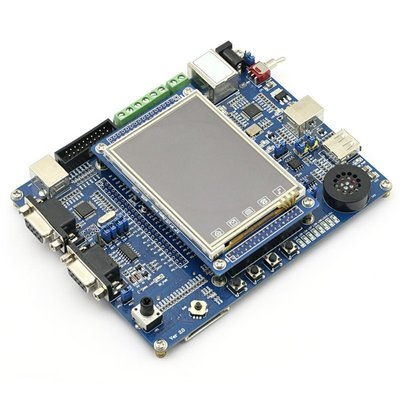
\includegraphics{./img/landTiger}
\caption{Mikrokontroler LandTiger wraz z wyświetlaczem. \cite{landtigerDesc}}
\end{figure}

Mikrokontroler LandTiger oparty na LPC1768 został wyprodukowany przez firmę PowerMCU i można go zakupić od wielu dostawców na eBay lub innych serwisach świadczących usługi zakupów przez internet. Średni koszt waha się w okolicach \$70 za płytkę wraz z wyświetlaczem LCD 3,2 cala o rozdzielczości 320x240 pikseli, z zasilaczem oraz zestawem kabli. \cite{landtigerDesc}
\newline
Funkcjonalności:
\begin{itemize} %[label=(\alph*)]
\item 2 porty RS232, jeden z nich wspiera ISP (In-system Programming),
\item 2 interfejsy magistrali CAN (Controller Area Network),
\item interfejs RS485,
\item interfejs Ethernetowy RJ45-10/100M,
\item przetwornik cyfrowo-analogowy (DAC) wraz wmontowanym głośnikiem (wyjściem interfejsu) oraz sterownikiem dźwięku (LM386),
\item przetwornik analogowo-cyfrowy (ADC) wraz z wbudowanym potencjometrem (wejściem interfejsu),
\item Kolorowy 3,2 cala (lub 2,8 cala) dotykowy wyświetlacz LCD o rozdzielczości 320x240 pikseli,
\item interfejs USB2.0 (USB Host oraz USB Device),
\item interfejs kard SD/MMC,
\item interfejs I2C połączony z 2Kbit pamięcią EEPROM,
\item interfejs SPI połączony z 16Mbit pamięcią flash,
\item 2 user keys, 2 function keys,
\item 8 diód typu LED,
\item pięciokierunkowy joystick,
\item wsparcie dla pobierania ISP,
\item pobieranie z użyciem JTAG, interfejs dla debugowania,
\item zintegrowany emulator kompilacji JLINK - wspiera możliwość debugownia online (po kablu USB podłączonym do PC) dla środowisk deweloperskich tj. KEIL, IAR, CooCox i innych,
\item dodatkowe 5V port zasilający (możliwe jest też za pomocą portu USB.
\end{itemize}

\begin{figure}[h]
\centering
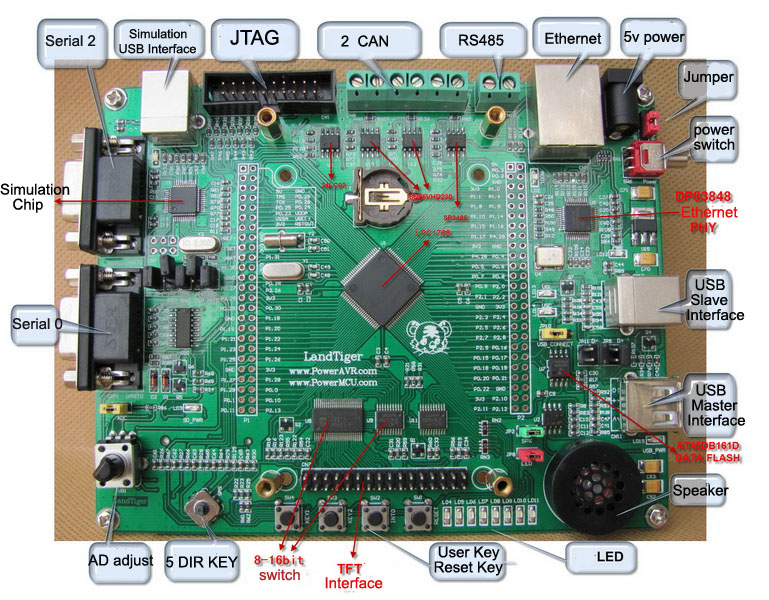
\includegraphics{./img/landTiger3}
\caption{Mikrokontroler LandTiger wraz z opisem poszczególnych elemetnów. \cite{landTiger3}}
%example\caption{Krzywa plastyczności wyrażająca zależność odkształcenia od naprężenia podczas rozciągania materiału ciągliwego \cite{bib7}} 
\end{figure}
LandTiger jest oparty na LPC1768. Wbudowany hardware wspiera ISP aby umożliwić załadowanie kodu (z użyciem bin2hex oraz flashmagic).
%\newline
Alternatywą jest to, że kod może zostać załadowany za pomocą emulatora JLINK JTAG/SWD lub za pomocą zewnętrznego urządzenia JTAG.
\newline
Port COM1 (UART0) wspiera komunikację z PC w obie strony. Wszelkie funkcje portu USB są wspierane z minimalnymi zmianami w oprogramowaniu. Podobnie jest z Ethernetem, z niewielkimi  zmianami w oficjalnym kodzie dla LPC1768, kod jest w stanie się uruchomić na LandTigerze.
\newline
\indent Wyświetlacz LCD jest oparty na kontrolerze SSD1289. Wyświetlacz może zostać odłączony od płyty. Używa on 8-bitowej magistrali \(P2_0..P2_7\). Kontroler ekranu dotykowego jest dostarczony razem z modułem wyświetlacza. Interfejs pomiędzy ekranem dotykowym a LPC1768 jest możliwy dzięki SPI.
\newline
Główne różnice pomiędzy LandTigerem a LPC1768:
\begin{itemize} % [label=(\alph*)]
\item płyta po podłączeniu do PC nie pokazuje się jako zewnętrzne urządzenie magazynujące,
\item aby ściągnąć nowe pliki binarne należy użyć ISP lub JTAG,
\item brak wsparcia dla serialowego portu po linku USB, należy używać RS232 lub portu USB,
\item brak wsparcia dla logicznego systemu plików,
\item brak wsparcia dla 4 diód typu LED (istnieje możliwość użycia inncyh).
\end{itemize}

%Parametry mikrokontrolera LandTiger wydawały się być zadowalające aby wykonać na nim testy. Niestety, jak się podczas wykonywania testów okazało (a zostało dokładniej opisane w rozdziale \ref{resultsChapter}) pomimo wlutowanego złącza wspierającego USB2.0, chip na kontrolerze wspiera standard USB1.1. Dzięki wynikom uzyskanym z użyciem LandTiger'a możemy obliczyć możliwości gdyby wsparcie USB2.0 na kontrolerze było zaimplementowane.
%\afterpage{\blankpage}
Przed rozpoczęciem projektowania klas należało zaznajomić się jak przedstawione jest USB na schemacie ideowym płytki LandTiger (Rys. \ref{fig:usbSchema}).
\begin{figure}[H]
\centering
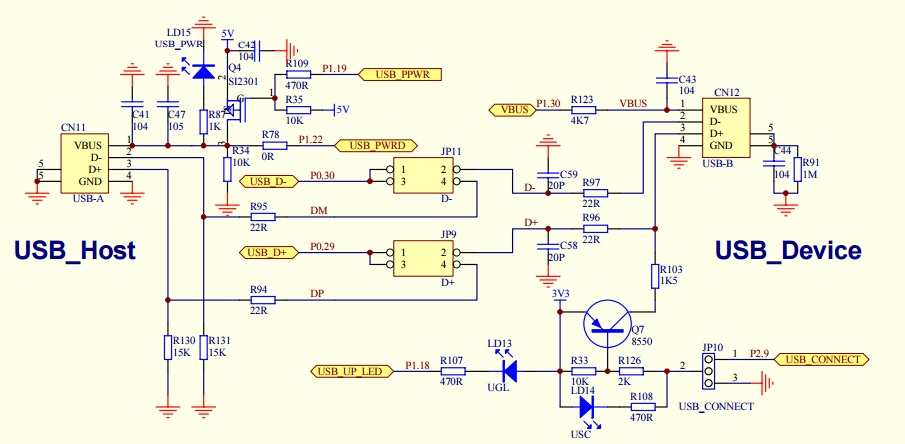
\includegraphics[width=1\textwidth]{./img/usbSchema}
\caption{Schemat ideowy USB na płytce LandTiger.\cite{landtigerDesc}} 
\label{fig:usbSchema}
\end{figure}
\noindent W projekcie wykorzystywano jedno z przedstawionych na rysunku złączy. Był nim USB\_Device, a co za tym idzie wszystkie zworki musiały zostać odpowiednio przestawione aby umożliwić jego działanie (JP9, JP10, JP11). Na schemacie widoczne jest, iż jest to złącze typu B (grubsze). Składa się z czterech pinów:
\begin{itemize}
\item Pin 1 - VBUS, odpowiada za dostarczenie zasilania +5V,
\item Pin 2 - terminal do przesyłania odwróconego sygnału (D-),
\item Pin 3 - terminal do przesyłania sygnału (D+)
\item GND - uziemienie
\end{itemize}
\noindent Istotne jest to aby długości D+ oraz D- były takie same, wtedy sygnał pokonuje dokładnie takie same odległości i zapewniona zostaje integralność. W wypadku kiedy odległości są różne mogą wystąpić różnego rodzaju błędu związane z wyeliminowaniem zakłóceń (eliminacja zakłóceń opisana dokładniej w rozdziale \ref{ch:motivationAndBasics}). Na schemacie różnica jest niezauważalna. Dodatkowo na poszczególnych liniach użyto filtry dolnoprzepustowe aby wyeliminować z widma sygnału częstotliwości powyżej częstotliwości Nyquista, czyli częstotliwości z jaką (w wypadku elektroniki) możliwy jest odczyt sygnału bez błędów, takich jak nakładania się składowych widmowych sygnału o wyższych częstotliwościach (niż częstotliwość Nyquista) na składowe o niższych częstotliwościach.
\newline
\indent Rozdział ukazuje, że Mikrokontroler LandTiger jest rozbudowanym urządzeniem zawierającym szereg różnego rodzaju funkcjonalności. Doskonale nadaje się jako urządzenie dla osób, które nie miały zbyt dużej styczności z programowaniem embedded, a jego przejrzyste API oraz dokumentacja pozwala na szybkie wdrożenie się w środowisko. \cite{landtigerDesc, embeddedC, embeddedSystems, bootstrapLinUSB}
%\afterpage{\blankpage}
\chapter{Implementacja}
\label{implementationChapter}
Implementacja opiera się na wykorzystaniu prostych podstawowych funkcji z biblioteki libUsb. Rozwiązania zostały obudowane w odpowiednie klasy wraz z zastosowaniem polimorfizmu, aby uzyskać możliwość łatwego dodawania nowych udoskonaleń. Diagram klas użytych w projekcie znajduje się na rysunku \ref{fig:classDiagram}. Doskonale pokazuje to łatwość rozszerzalności o nowe funkcjonalności aplikacji. Jeżeli w przyszłości uda się opracować nowy sposób przesyłania danych, można rozszerzyć klasę Mode o tą funkcjonalność. Opis poszczególnych klas wraz z użytymi metodami znajduje się w poniższych podrozdziałach. Klasa abstrakcyjna Mode udostępnia bardzo podstawowe metody służące do inicjalizacji oraz czyszczenia zasobów. W wypadku tworzenia własnego trybu oraz konieczności innej inicjalizacji (lub zwalniania zasobów) należy dostarczyć własną implementacje tych metod. Konieczne jest dostarczenie implementacji testu.
\begin{figure}[H]
\centering
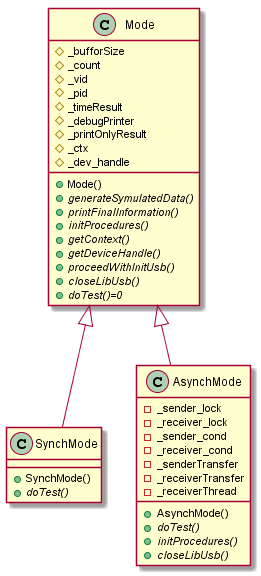
\includegraphics[width=0.4\textwidth]{./img/classDiagram}
\caption{Diagram klas projektu.}
\label{fig:classDiagram}
\end{figure}
Głównym założeniem implementacyjnym było stworzenie jak najłatwiej rozszerzalnego i zrozumiałego interfejsu. W takim celu powstała klasa Mode (dokładniejszy opis poniżej). Klasa zawiera w sobie najważniejsze podstawowe implementacje funkcjonalności libUSB jednocześnie pozwalając na łatwą rozszerzalność tych funkcjonalności (np. w wypadku AsynchMode funkcjonalność ta została rozszerzona). Dodatkowo wymagana jest implementacja samego testu (metoda doTest()), implementacje pomiędzy SynchMode oraz AsynchMode znacząco się różnią. Jak wspomniane zostało powyżej, najistotniejsze w projekcie jest to, że rozwijając projekt wystarczy przeciążyć klasę Mode, rozwijając odpowiednio funkcjonalności oraz dodając odpowiednią część wykonawczą testu.
\newline
\indent Cele implementacyjne zostały całkowicie zrealizowane w przedstawionym projekcie. Klasa Mode pozwala na przyszłą rozbudowę funkcjonalności i testowanie innych sposobów przesyłu danych. Natomiast klasy SynchMode oraz AsynchMode zawierają implementację spełniającą wymagania projektu. Poniższe podrozdziały zawierają szczegóły techniczne poszczególnych elementów implementacji. Wszelkie listingi poszczególnych metod znajdują się w dodatku C.
\section{Klasa Mode}
Klasa Mode jest nadzbiorem funkcjonalności. Obudowuje ona podstawowe funkcjonalności takie jak:
\begin{itemize}
\item inicjalizacja
\subitem pobieranie kontekstu,
\subitem pobieranie uchwytu urządzenia,
\subitem rejestracja interfejsu,
\item oczyszczanie pamięci.
\end{itemize}
Definicja zawiera również czysto wirtualną metodę doTest(), której odpowiednie implementacje w obiektach dziedziczących dostarcza funkcjonalności testom.

\subsection{Metoda getContext}
W listingu \ref{lst:Mode_getContext}. przedstawione zostało ciało metody getContext() klasy Mode.
Metoda nie przyjmuje żadnego argumentu, natomiast inicjalizuje kontekst i zapamiętuje go jako składową klasy. W rozdziale \ref{libUsbChapter} wspomniane zostało iż możliwe jest używanie kontekstu domyślnego, wtedy zamiast użycia libusb\_init() należałoby przypisać wskaźnikowi do kontekstu wartość równą NULL. 
Aby używać domyślnego kontekstu należy mieć pewność iż aplikacja/wątek jest jedynym użytkownikiem libUSB.
W wypadku niepoprawnego działania wyrzucany jest błąd (ważne aby był przechwycony w funkcji main).
\subsection{Metoda getDeviceHandler}
Metoda nie przyjmuje żadnego argumentu. Jej zadaniem jest ustawienie uchwytu do urządzenia na podstawie jego vendorId oraz productId. W wypadku niepowodzenia zostanie zgłoszony odpowiedni błąd (np. braku podłączonego i uruchomionego mikrokontrolera).
Ciało funkcji zostało przedstawione w Listingu \ref{lst:Mode_getDeviceHandle}.
\subsection{Metoda proceedWithInitLibUsb}
Metoda ta odpowiedzialna jest za dokończenie procedur inicjalizacyjnych. Ciało metody zostało przedstawione w Listingu \ref{lst:Mode_proceedWithInitLibUsb}. Metoda sprawdza dodatkowo czy sterownik jądra kernela jest aktywny, dla platformy Windows funkcja zwróci wartość błędu, która będzie równa wartości enumerycznej LIBUSB\_ERROR\_NOT\_SUPPORTED (!= 1) i zachowa się analogicznie jak w wypadku nieaktywnego sterownika w systemie UNIX (warunek będzie niespełniony).
Kolejnym krokiem jest rezerwacja przez program konkretnego interfejsu za pomocą funkcji libusb\_claim\_interface.
W wypadku niepoprawnego działania metoda wyrzuci runtime\_error, który należy obsłużyć  w funkcji main().


\subsection{Metoda initProcedures()}
Metoda przedstawiona w listingu \ref{lst:Mode_initProcedures}. odpowiada za wywołanie procedur inicjalizacji w odpowiedniej kolejności.
\subsection{Metoda closeLibUsb}
Metoda przedstawiona w Listingu \ref{lst:Mode_closeLibUsb} odpowiada za zwolnienie interfesju oraz zasobów uprzednio zajętych na czas testu.

\section{Klasa SynchMode}
Klasa SynchMode jest odpowiedzialna za konfigurację USB dla przesyłu synchronicznego. Jest rozszerzeniem klasy Mode.
\begin{lstlisting}[caption={Deklaracja klasy SynchMode},label={lst:CSynchMode}]
class SynchMode : public Mode
{
public:
	SynchMode(int bufforSize, unsigned count, int vid, int pid, bool printOnlyResult);
	virtual ~SynchMode();
	virtual int doTest() override;
};
\end{lstlisting}
Używa ona wszystkich domyślnych ustawień, Przeciążona jest tylko metoda odpowiadająca za poprawne wykonanie testu.
\subsection{Metoda doTest}
Metoda jest odpowiedzialna za wykonanie podstawowego pomiaru czasu przepływu danych w obie strony, pomiędzy PC a mikrokontrolerem.
Została zaprojektowana w taki sposób aby konkretny bufor danych został wysłany oraz odebrany określoną ilość razy i zwrócony przedział czasowy w jakim udało się to uzyskać. Powodem wysyłania/odbierania danych określoną ilość razy jest fakt sporych ograniczeń jeśli chodzi o chip wbudowany w płytę LandTiger. Fragment metody został przedstawiony w listingu \ref{lst:SynchMode_doTest}.
\begin{lstlisting}[caption={Fragment metody SynchMode::doTest()},label={lst:SynchMode_doTest}]
int SynchMode::doTest()
{
//...
		int sendStatus = libusb_bulk_transfer(_dev_handle, (2 | LIBUSB_ENDPOINT_OUT), data_out, _bufforSize, &howManyBytesIsSend, 0); 
//...		
		int readStatus = libusb_bulk_transfer(_dev_handle, (2 | LIBUSB_ENDPOINT_IN), data_in, _bufforSize * sizeof(unsigned char), &howManyBytesReceived, 0);
//...
}
\end{lstlisting}
\section{Klasa AsynchMode}
Klasa AsynchMode odpowiada za konfigurację USB dla przesyłu asynchronicznego. 

\begin{lstlisting}[caption={Deklaracja klasy AsynchMode},label={lst:CAsynchMode}]
class AsynchMode : public Mode
{
public:
	AsynchMode(int bufforSize, unsigned count, int vid, int pid, bool printOnlyResult);
	virtual ~AsynchMode();
	virtual int doTest() override;
	virtual void initProcedures() override;
	void closeLibUsb() override;
//..
};
\end{lstlisting}
Klasa zawiera wzbogaconą inicjalizację o alokację transferów (wysyłającego oraz odbierającego) oraz inicjalizację mutexów.
Dodatkowo został utworzony dodatkowy namespace ułatwiający obsługę callbacków. Znajduje się w nim zarówno obsługa wątku nasłuchującego jak i obsługa poszczególnych zdarzeń.
\subsection{Metoda initProcedures oraz closeLibUsb}
W wypadku asynchronicznego przesyłania danych należy wykonać kilka dodatkowych operacji inicjalizacyjnych. Są to alokacje transferów oraz inicjalizacja mutexów.
Calość widoczna w listingu \ref{lst:AsynchMode_initProcedures}.
Analogicznie sytuacja przedstawia się w wypadku zwalniania zasobów. Dodatkową czynnością jest usunięcie mutexów oraz zwolnienie transferów. Całość dostępna w listingu \ref{lst:AsynchMode_closeLibUsb}.
\subsection{Metoda doTest}
Podobnie jak w wypadku synchronicznego mechanizmu tak i teraz należy dostarczyć implementację metody doTest(). Natomiast jej działanie jest odmienne, ponieważ polega na wystartowaniu drugiego wątku nasłuchującego odpowiedzi. Całość synchronizowana jest za pomocą mutexów (listing \ref{lst:AsynchMode_doTest} oraz \ref{lst:ThreadHelper}).
\begin{lstlisting}[caption={Metoda AsynchMode::doTest()},label={lst:AsynchMode_doTest}]
int AsynchMode::doTest()
{
//...
	libusb_fill_bulk_transfer(_senderTransfer, _dev_handle, (2 | LIBUSB_ENDPOINT_OUT), data_out, _bufforSize, ThreadHelper::cb_send, &transferStatus, 0);
	libusb_fill_bulk_transfer(_receiverTransfer, _dev_handle, (2 | LIBUSB_ENDPOINT_IN), data_in, _bufforSize, ThreadHelper::cb_read, &transferStatus, 0);
//..
	if(pthread_create(&_receiverThread, NULL, ThreadHelper::receiverThread, &transferStatus) != 0)
	{
		throw std::runtime_error("Error creating listener thread.");
	}
//... 
		pthread_mutex_lock(&_sender_lock);
		while(transferStatus.waitForSender){
			pthread_cond_wait(&_sender_cond, &_sender_lock);
		}
		transferStatus.waitForSender = 1;
		pthread_mutex_unlock(&_sender_lock);
		transferStatus.particularSendComplete = 0;
		libusb_submit_transfer(_senderTransfer);
	//...
}

\end{lstlisting}

\section{Korzystanie z poszczególnych interfejsów}
Kod przedstawiony w Listingu \ref{lst:main} doskonale ukazuje prostotę korzystania z libUSB. Użytkownik zobligowany jest do wprowadzenia wielkości bufora danych oraz liczbę określającą ilość powtórzeń z jaką testowa aplikacja wyśle wygenerowane dane (o rozmiarze podanego bufora) do mikrokontrolera. Następnie zostaje wykonana inicjalizacja z użyciem wyżej wymienionych interfejsów (synchronicznego lub asynchronicznego na podstawie parametru).
\begin{lstlisting}[caption={Przykład użycia interfejsu synchronicznego lub asynchronicznego w zależności od parametryzacji},label={lst:main}]
int main(int argc, char* argv[])
{
	//..
	try 
	{
		std::unique_ptr<Mode> mode;

		if(selectedMode == 'A')
			mode.reset(new AsynchMode(bufforSize, count, LAND_TIGER_VID, LAND_TIGER_PID, printOnlyResult));
		else 
			mode.reset(new SynchMode(bufforSize, count, LAND_TIGER_VID, LAND_TIGER_PID, printOnlyResult));
		mode->initProcedures();
		mode->doTest();
		mode->printFinalInformation();
		mode->closeLibUsb();
	} catch (std::runtime_error& e)
	{
		std::cout << e.what() << std::endl;
	}

	return 0;
}

\end{lstlisting}
\subsection{Parametryzacja}
\noindent Aby ułatwić uruchamianie poszczególnych testów wprowadzono możliwość sparametryzowania wejścia aplikacji:
\begin{lstlisting}[caption={uruchomienie testu}]
use: libusb [S/A] <bufforSize> <fullDataSize> optional:<printOnlyResult>
\end{lstlisting}
\begin{itemize}
\item S/A - należy wybrać czy chcemy wykonać test w trybie Synchronicznym czy Asynchronicznym,
\item bufforSize - rozmiar bufforu danych jaki chcemy przeznaczyć dla jednej paczki danych [B],
\item fullDataSize - całkowity rozmiar danych do wysłania [B],
\item printOnlyResult - opcjonalny parametr w wypadku ustawienia na wartość '1' pozwala na łatwe zebranie wyników bez zbędnych informacyjnych wiadomości (same dane). 
\end{itemize}
\section{Implementacja pomocnicza}
\label{sch:additionalImplementation}
Do implementacji pomocniczej należy klasa ułatwiająca wywoływanie aplikacji celem zebrania wyników. Jest ona zaprojektowana jako prosta, posiadająca przeładowany operator dodawania do strumienia danych. W wypadku tego projektu, dla normalnego działania aplikacji operator pozwala na wypisanie dowolnych danych, ale w wypadku włączenia zbierania danych w postaci kolumnowej ta klasa nie pozwoli na to (całość dostępna w listingu\ref{lst:CDebugPrinter}.). Działanie jest widoczne, jeżeli wywołanie aplikacji zostanie odpowiednio sparametryzowane:
\begin{lstlisting}[caption={Uruchomienie testu}]
use: libusb [S/A] <bufforSize> <fullDataSize> optional:<printOnlyResult>
\end{lstlisting}
bez ostatniego argumentu, w wypadku wykonania tego fragmentu kodu: 
\begin{lstlisting}[caption={Wypisywanie w zależności od argumentu wywołania aplikacji}]
debugPrinter << "It is impossible to send " << fullDataSize << "B using " << bufforSize << "B, to simplify application work sending " << (++count) * bufforSize << "B\n";
\end{lstlisting}
aplikacja wypisze powyższy tekst, natomiast w wypadku wywołania aplikacji wraz z ostatnim opcjonalnym argumentem <printOnlyResult>=1 spowoduje, że przeładowany operator klasy wspomnianej w listingu \ref{lst:CDebugPrinter}. zablokuje wypisywanie tekstu.
Klasa została stworzona tylko po to aby ułatwić przyszłe zbieranie wyników.
\afterpage{\blankpage}
\chapter{Testy wydajności oraz ich rezultaty}
\label{resultsChapter}
\indent Oprogramowanie zostało poddane dogłębnym testom systemowym, mającym na celu zweryfikowanie poprawności działania aplikacji oraz jej zgodności z wymaganiami. Wykonywano je na każdym etapie programowania aby uniknąć jakichkolwiek nieumyślnych interakcji w rezultaty działających uprzednio funkcjonalności. Ważne było aby środowisko testowe było znane. W przypadku tego projektu jest to mikrokontroler LandTiger opisany dokładniej w rozdziale \ref{microcontrollerChapter} oraz komputer osobisty o parametrach przedstawionych w tabeli \ref{tbl:pcParameters}.
\begin{table}[H]
\centering
\begin{tabular}{|c|c|}
\hline
	\rowcolor[gray]{0.8}
	Typ procesora & DualCore Intel Core i3 350M, 2266 MHz (17 x 133) \\ \hline
	
	Pamięć & 6GB \\ \hline
	 \rowcolor[gray]{0.8}
	 Dysk fizyczny & WDC WD3200BPVT-80ZEST0  (298 GB) \\ \hline
	USB & 2.0 \\ \hline
\end{tabular}
\captionof{table}{Podstawowe parametry komputera na którym wykonywane zostały testy}
%source: 
\label{tbl:pcParameters}
\end{table}
\noindent Istotnym elementem wymagań było to aby aplikacja była wieloplatformowa, włączając przede wszystkim system Windows oraz systemy z rodziny Linux. Testy zostały wykonane na systemie Windows 8.1 Pro oraz na Linux Ubuntu 14.04.
\noindent Analizując poniższe wyniki testów należy mięć na uwadze poniższe fakty i założenia:
\begin{enumerate}
\item Początkowym celem było uzyskanie prędkości nie mniejszej niż 140 Mbit/s co daje 17,5 MB/s w obu kierunkach.
\item Zarówno komputer osobisty jak i płytka LandTiger posiada wbudowane złącze żeńskie standardu USB2.0 (komputer złącze typu A, natomiast płytka złącze typu B).
\item Jak się okazało podczas tworzenia projektu płytka LandTiger, pomimo wlutowanego złącza USB2.0, nie jest w stanie obsłużyć tego standardu. Spowodowane jest to tym iż chip na płycie wspiera jedynie standard USB1.1.
\item warunkiem koniecznym udanego testu jest niestety wsparcie minimum USB2.0.
\end{enumerate}
\section{Testy jednostkowe}
\indent Testy jednostkowe miały na celu sprawdzenie poprawności działania poszczególnych metod oraz klas projektu. Dodatkowo chroniły proces tworzenia nowych funkcjonalności aby nie ingerowały w działanie uprzednio napisanych. Testy jednostkowe tworzone były równolegle z programowaniem poszczególnych funkcjonalności dzięki czemu udało się zadbać o całkowitą spójność projektu.
\section{Testy akceptacyjne i regresyjne}
\indent Testy akceptacyjne mają za zadanie sprawdzenie czy dana aplikacja spełnia wymagania i warunki oraz potwierdzić czy w testowym środowisku aplikacja działa poprawnie. Były one wykonywane równolegle z procesem tworzenia oprogramowania dzięki czemu udało się zidentyfikować problemy w locie. Zostały wykonane na zasadzie black box testing. Metodologia ta polega na tym, iż tester testuje konkretną, zaimplementowaną funkcjonalność bez wglądu w kod produkcyjny, opierając się tylko na wymaganiach danej funkcjonalności. Jest to o tyle słuszne, w wypadkach kiedy testy te wykonywane są przez inną osobę, niż osobę która implementowała funkcjonalność, ponieważ programista może podświadomie wymusić tylko te zachowania aplikacji, które zostały zaimplementowane przez niego, natomiast osoba opierająca się tylko na wymaganiach sprawdzi całość.
%\indent Testy zostały przeprowadzone z użyciem prostej aplikacji w dwóch trybach: synchronicznym i asynchronicznym. Przedstawione poniżej wyniki wraz z krótką interpretacją przekazują zarys doświadczenia. Celem pracy było uzyskanie prędkości nie mniejszej niż 140 MBit/s co jest równe 17,5 MB/s.
%\newline
%\indent Niestety okazało się iż mikrokontroler LandTiger pomimo wlutowanego gniazda USB2.0 nie jest w stanie obsłużyć tego standardu. Powodem tego jest to iż chip na płytce jest w stanie obsłużyć tylko standard USB1.1.
%\newline
%\indent Powodem dla którego mikrokontroler działa pomimo obsługi USB1.1 (a nie jak wspomniano USB2.0) jest to że wlutowane gniazdo ustandaryzowane jako USB2.0 jest wstecznie kompatybilne (więcej informacji w rozdziale \ref{USBStandardChapter}).
%\newline
\section{Zestawienie wyników}
\indent Zebrane wyniki możemy skategoryzować według: ilości przesłanych danych, szybkości przesyłu danych z komputera osobistego do kontrolera, szybkości przesyłu danych z kontrolera do komputera osobistego, szybkości przesyłu w obie strony. Kluczowym elementem jest tutaj wielkość buffora, czyli ilości danych możliwych do wysłania/odebrania w jednym tiku zegara.
\newline
\indent Według założeń USB 2.0 jest w stanie obsłużyć oczekiwane 140Mbit/s (17,5 MB/s). Wykres przedstawiony na Rys. \ref{fig:speedTest} doskonale to obrazuje.
\begin{figure}[H]
\centering
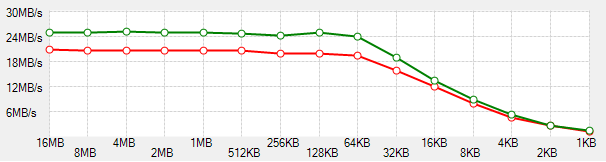
\includegraphics[width=0.9\textwidth]{./img/speedTest}
\caption{Zależność prędkości przesyłu danych od wielkości bufora.}
\label{fig:speedTest}
\end{figure}
Rysunek \ref{fig:speedTest} przedstawia wykres prędkości wysyłania oraz odbioru danych w zależności od bufora danych (bufor maleje)\footnote{dane uzyskane dzięki programowi USB Flash Benchmark\cite{USBFlashBenchmark}}. Na wykresie zielona linia przedstawia odczyt danych z użyciem interfejsu USB2.0 natomiast czerwona przedstawia prędkość wysyłania danych. Wybrane wyniki w formie tekstowej są częścią załącznika B niniejszej pracy. Etapem godnym uwagi jest zachowanie wykresu w momencie gdy buffor danych wynosi 64KB, jest to ostatnia stabilna wartość buffora, która umożliwiałaby spełnienie wymagań projektu. W wypadku wartości 32KB widoczny jest jeszcze spełnienie warunku ale tylko dla danych wysyłanych (zielona linia). Pozostałe wartości buffora nie spełniają warunków projektu.
\newline
\indent Podczas testów akceptacyjnych równolegle z developmentem okazało się iż płytka użyta w projekcie a dokładniej opisana w rozdziale \ref{microcontrollerChapter} wspiera na swoim chipie jedynie standard USB1.1 pomimo wlutowanego złącza USB2.0. Niestety w wypadku USB1.1 jest to 64B. Większość wyników została wygenerowana za pomocą programu, który nie pozwalał na przekroczenie dopuszczalnego przez LandTiger'a bufforu (tak jak w przypadku Rys. \ref{fig:S_107374200Receive} oraz innych)
\newline
\begin{figure}[H]
{
\centering
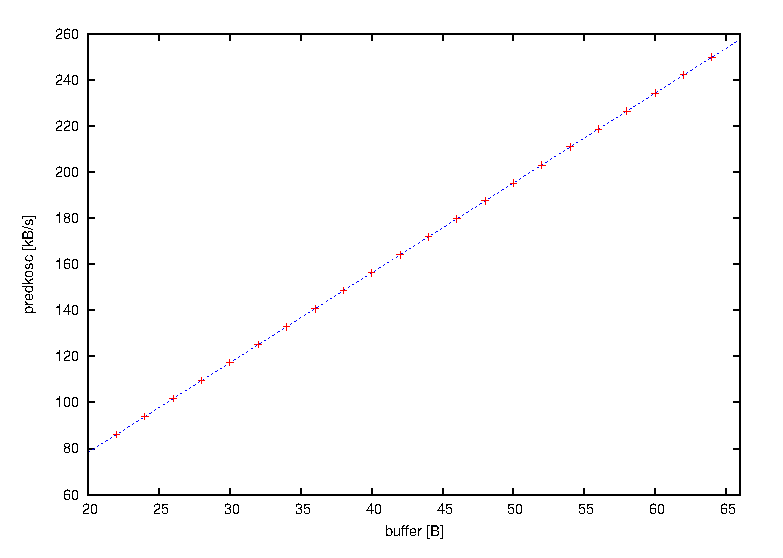
\includegraphics[width=1\textwidth]{./img/S_107374200Receive}
\caption{Wykres ilustrujący prędkość przesyłu danych w zależności od bufora dla danych wielkości ok. 102MB (tryb synchroniczny).}
\label{fig:S_107374200Receive}
%\end{figure}
}
\end{figure}
%%todo
\noindent Na Rys. \ref{fig:S_107374200Receive} widoczny jest wyraźny wzrost szybkości wysyłania oraz odbierania danych wraz ze zwiększeniem bufora. Jest to doświadczenie wykonane na stosunkowo małym buforze, spowodowane jest to ograniczeniami płytki LandTiger. Można zaobserwować liniową zależność pomiędzy zobrazowanymi wielkościami. Różnice pomiędzy prędkością wysyłania a odbierania są niezauważalne przy tak małej ilości danych.
%44\begin{figure}[htpb]

%\begin{figure}[H]
%{
%\centering
%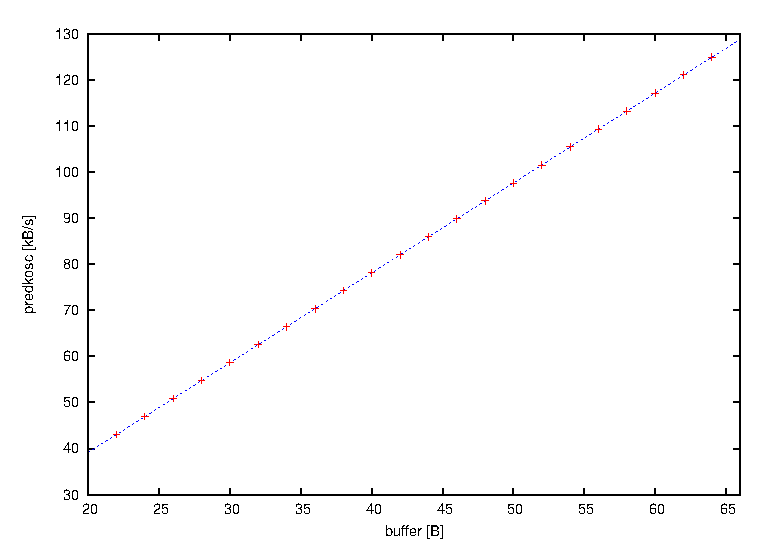
\includegraphics[width=0.75\textwidth]{./img/S_107374200SendReceive}
%\caption{TODO S\_107374200SendReceive.jpg}
%\label{fig:S_107374200SendReceive}
%\end{figure}
%}
%\end{figure}
%%%%%%
\begin{figure}[H]
{
\centering
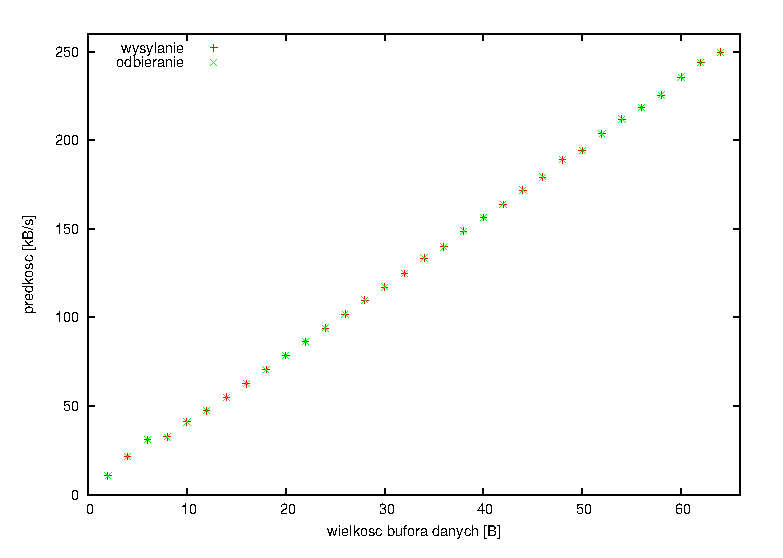
\includegraphics[width=1\textwidth]{./img/S_10737420Receive}
\caption{Wykres ilustrujący prędkość wysłania danych w zależności od buffora wielkości ok. 10MB (tryb synchroniczny).}
%\end{figure}
\label{fig:S_10737420Receive}
}
\end{figure}
\noindent W wypadku wysyłania nieco mniejszej próbki danych prędkość obrazuje się jako nieco mniej stabilna. Całość widoczna jest na Rys. \ref{fig:S_10737420Receive}. Podobnie jak w poprzednim przypadku (dla większej ilości danych), nie ma widocznej różnicy pomiędzy prędkością wysyłania danych jak i odbieranych (Rys. \ref{fig:S_107374200Receive}).
\newline
\indent Wszystkie powyższe wykresy zostały wygenerowane z użyciem mechanizmu synchronicznego. Oznacza to, że obsługa wysyłania oraz odbierania danych zrealizowana została za pomocą wbudowanych bibliotek, co z punktu widzenia kodu aplikacji  realizuje taka sama paczka danych wysłanych oraz odebranych. Podsumowując powyższe wyniki można uznać metodę synchroniczną za nieskuteczną dla standardu USB1.1. Oczekiwane wyniki nie zostały w tym wypadku uzyskane. Mechanizmem blokującym jest wielkość bufora danych przy wysyłaniu lub odbieraniu danych (64B). Jest to zdecydowanie za mało aby ta metoda w tym wypadku była skuteczna ale porównując otrzymane wyniki z teoretycznymi (Rys. \ref{fig:speedTest} oraz dodatek B) otrzymanymi z użyciem USB benchmark, gdzie najmniejsza wielkość bufora wynosiła 1kB oraz wartość otrzymana oscylowała w okolicach 1,26MB-1,36MB można założyć iż wartości otrzymane z użyciem metody synchronicznej są jak najbardziej poprawne, a ograniczeniem, które nie pozwala na uzyskanie oczekiwanych wartości jest jedynie konieczność użycia standardu USB1.1.
%Synchroniczne wysyłanie danych nie należy do najbardziej efektywnych metod (dotyczy USB1.1), ponieważ wielkość bufora danych (64B) ograniczona poprzez standard USB1.1 
%Każda operacja zwraca status i ten status musi być weryfikowany aby zlokalizować ewentualny błąd.
%%%%% Asynch
\newline
\indent Zupełnie innym podejściem charakteryzuje się metoda asynchroniczna w której korzysta się z nieblokujących metod. Istotne jest, aby zauważyć, że o synchronizacje dba programista (ponieważ po łączu w jednym czasie mogą przebiegać dane tylko w jedną stronę). Na podstawie przeprowadzonego doświadczenia można stwierdzić, że implementacja była dużo bardziej kosztowna i wymagała przeznaczenia więcej czasu aby zadbać o poprawną synchronizacje danych. Niemniej to ona doprowadziła do większej kontroli nad zarządzaniem przełączania wysyłania oraz odbierania danych. W wypadku przesyłanych danych z wykorzystaniem LandTiger'a, a co za tym idzie wykorzystaniem jedynie dostępnego rozmiaru buforu danych wielkości 64B, zmiany są praktycznie niezauważalne.
\begin{figure}[H]
{
\centering
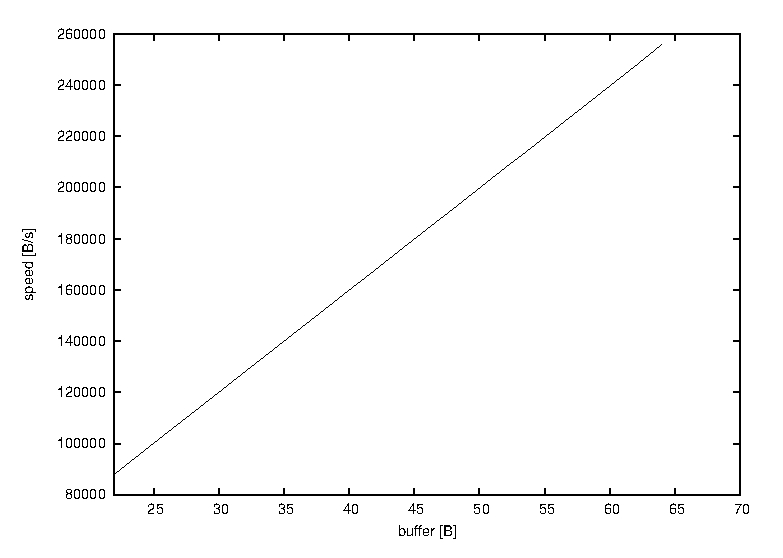
\includegraphics[width=1\textwidth]{./img/A_107374200Receive}
\caption{Wykres ilustrujący prędkość wysyłania danych w zależności od buffora (tryb asynchroniczny).}
\label{fig:A_107374200Receive}
}

\end{figure}

\noindent Jak widać na Rys. \ref{fig:A_107374200Receive} zależność liniowa również występuje dla tej ilości danych jak przy przesyle asynchronicznym. Sytuacja ta występuje zarówno w wypadku odbierania jak i wysyłania danych metodą asynchroniczną. Wykres jest liniowy jak jego odpowiednik z metody synchronicznej (Rys. \ref{fig:S_107374200Receive}) a wyniki są bardzo zbliżone do siebie.

%%%%%%

\begin{figure}[H]
{
\centering
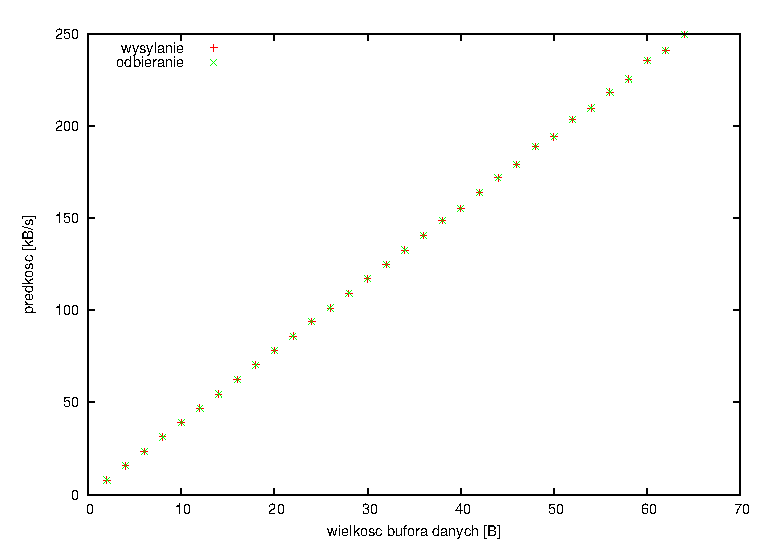
\includegraphics[width=1\textwidth]{./img/A_10737420Receive}
\caption{Wykres ilustrujący prędkość przesyłu danych w zależności od wielkości bufora danych dla danych wielkości ok. 10MB (tryb asynchroniczny).}
\label{fig:A_10737420Receive}
}
\end{figure}

\noindent Jeśli przeprowadzimy testy dla mniejszej ilości danych to zauważalny jest brak liniowości takiego wykresu (Rys. \ref{fig:A_10737420Receive}). Spowodowane jest to zmniejszoną ilością wysyłanej próbki danych, przez co uzyskano mniejszą stabilność. \\
\indent Wysyłanie metodą Asynchroniczną również nie przyniosła oczekiwanych rezultatów. Porównując je do wartości zasymulowanych na początku rozdziału z użyciem USB benchmark, pozostawiają wiele do życzenia. Jednak jeśli ponowimy zestawienie wyników z teoretycznymi (podobnie jak to zostało to wykonane w wypadku metody Synchronicznej) to zauważymy pewną analogię iż gdyby istniała możliwość wykorzystania bufora większego niż dopuszczalny przez standard USB1.1, wyniki nie odbiegałyby od teoretycznych.
\indent Podsumowując, użycie bufora dopuszczalnego przez mikrokontroler LandTiger (czyli bufora nie większego niż 64B) nie pozwala na uzyskanie wyników zbliżonych do wartości pożądanej (140 MB/s) bez względu na to, czy korzystano z metody synchronicznej czy też asynchronicznej. W obu przypadkach dla bufora o wielkości 64B udało się uzyskać maksymalnie 250 kB/s. Wyniki teoretyczne (dodatek B) przedstawiają dla bufora wielkości 1kB wyniki rzędu 1,26MB/s - 1,36 MB/s. Oznacza to, że przy założeniach otrzymanej dotąd liniowości, prędkość ta zostałaby osiągnięta, w wypadku możliwości użycia bufora wielkości 1kB przez aplikację.
\newline
\noindent Dodatkowo została przeprowadzona symulacja z uwzględnieniem większego bufora danych, jednak w tym przypadku nie udało się uzyskać prawidłowego odbioru danych  po stronie kontrolera. Oznacza to, że te dane mogą zostać potraktowane jedynie jako przypuszczenia jak wyglądałby wykres gdyby dane były przetworzone prawidłowo. Poniższe (Rys. \ref{fig:S_bbuf1} oraz Rys. \ref{fig:S_bbuf2} wykresy przedstawiają wygenerowane wyniki.
\begin{figure}[H]
{
\centering
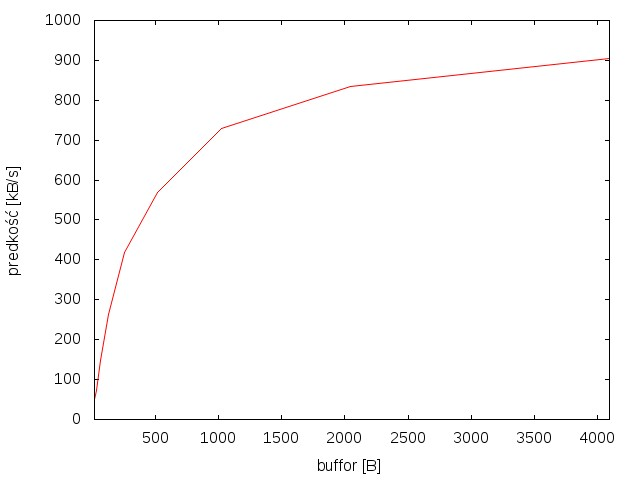
\includegraphics[width=1\textwidth]{./img/S_bbuf1}
\caption{Wykres ilustrujący zmianę prędkości przesyłania danych z użyciem bufora z przedziału 16 B - 4 kB.}
\label{fig:S_bbuf1}
}
\end{figure}
\noindent Powyższy wykres obrazuje zmianę prędkości wysyłania przy założeniu poprawnego odbioru danych po stronie kontrolera. Zależność liniowa całkowicie zaniknęła. Wartości rozmiaru bufora danych jest podwajana z każdym zgięciem krzywej (początkowa wartość 16 B, końcowa 4096 B = 4 kB), a więc rozbieżność przesyłu danych jest duża. Warto zauważyć iż pomimo dość dużego bufora danych prędkość nie przekroczyła 1 MB/s (max wartość 905,702 kB/s).
\begin{figure}[H]
{
\centering
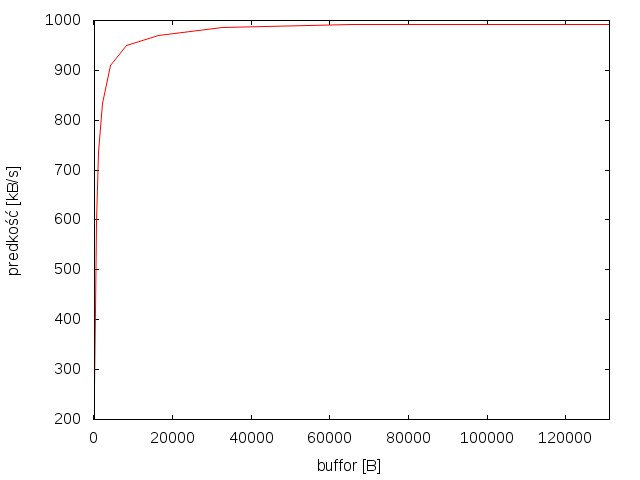
\includegraphics[width=1\textwidth]{./img/S_bbuf2}
\caption{Wykres ilustrujący zmianę prędkości przesyłania danych z użyciem bufora z przedziału 128B - 128kB.}
\label{fig:S_bbuf2}
}
\end{figure}
\noindent Powyższy wykres jest rozwinięciem poprzednika. Obrazuje zmianę prędkości na podstawie zasymulowanych danych oraz przy założeniach poprawnego odebrania danych przez mikrokontroler. Podstawową różnicą jest wielkość użytego bufora w tym przypadku. Został w nim użyty bufor o wartości minimalnej równej 128 B oraz maksymalnej równej 131072 B (128 kB). Bufor w każdym kroku był podwajany. Początkowo wartość uzyskiwanej prędkości wzrasta gwałtownie w każdym kroku, natomiast powyżej wartości 8 kB nie są już tak gwałtowne a wręcz przechodzi w coraz bardziej poziomy wzrost i dąży do wartości 1 MB/s. 
\newline
\indent Podsumowując całościowo wszystkie użyte metody w projekcie (Synchroniczna, Asynchroniczna) oraz zwykłą symulacje przesyłu większej ilości danych (pomimo braku możliwej obslugi po stronie mikrokontrolera) można założyć, iż w wypadku realizacji projektu z mikrokontrolerem obsługującym standard nowszy niż USB1.1 rezultaty oczekiwane zostałyby osiągnięte. Dodatkowo zestawiając metodę synchroniczną oraz asynchroniczną z wynikami teoretycznymi można śmiało potwierdzić, że jest to możliwe (zakładając iż trend wykresów nie ulegnie wielkiej zmianie). Należy mieć również na uwadze iż, mogą istnieć wszelkiego rodzaju problemy i zakłócenia trudne do namierzenia na styku złącza USB2.0 -> kabla USB2.0 -> złącza USB1.1 i na odwrót. Potwierdza to jedynie poprzednie założenia. Ostatnie dwa wykresy przedstawiają symulacje wysyłania danych z użyciem większego bufora danych ale bez poprawnej obsługi ich odbioru po stronie mikrokontrolera (ponieważ nie jest to możliwe z powodu ograniczeń płytki). Widoczne jest na nich, iż prędkość rośnie lecz zmienia trend z czysto liniowego w typowo logarytmiczny. Powodem są prawdopodobne zakłócenia wspomniane wcześniej, niemożliwość przetworzenia danych po stronie płytki, a co za tym aplikacja nie wie kiedy wysłanie partii danych się zakończyła i kiedy powinna rozpocząć wysyłanie kolejnej oraz inne obostrzenia USB1.1. Zestawiając do testów urządzenie obsługujące standard USB2.0, brak obsługi otrzymanych danych nie miałby miejsca co zapewniłoby płynność w przesyłaniu większej ilości danych i zapewne wykresy oparte na podobnych wartościach przedstawiałyby dane zgodne z teoretycznymi.

%Porównując wyniki do wartości zasymulowanych na poczatku rozdziału z wykorzystaniem pełnych funkcjonalności USB2.0 można założyć iż w wypadku braku ograniczeń USB1.1 istnieje możliwość powodzenia projektu.
\afterpage{\blankpage}
\chapter{Podsumowanie}
\label{ConclusionChapter}
\indent Celem projektu było przygotowanie oprogramowania umożliwiającego wysyłanie i odbieranie danych z wykorzystaniem złącza uniwersalnej magistrali szeregowej, czyli USB. Aby zrealizować projekt należało poznać standard USB i zrozumieć jego działanie, jak i innych, mniej lub bardziej zaawansowanych portów szeregowych. Istotne było zrozumienie różnic pomiędzy standardami wydanymi do dnia dzisiejszego jako podstawa teoretyczna do zrealizowania projektu. Projekt posiada zintegrowany system testowania funkcjonalności, aby zapobiec negatywnej ingerencji w istniejące już funkcjonalności.
\newline
\indent Najważniejszym krokiem podczas tworzenia projektu był wybór urządzenia testowego, czyli urządzenia na którym wykonywane były najważniejsze testy akceptacyjne. Wybór padł na mikrokontroler LandTiger, który został dokładniej opisany w rozdziale \ref{microcontrollerChapter}. Aplikacja została zaprojektowana w prosty i rozszerzalny sposób. Głównym punktem projektu jest klasa abstrakcyjna pełniąca podstawowe funkcje oraz posiadająca domyślne implementacje poszczególnych metod. Po tej klasie zostały podziedziczone dwie inne wprowadzające własne wersje implementacji testu, jak i w wypadku bardziej rozbudowanej klasy odpowiadającej za asynchroniczne przesyłanie danych, również inicjalizacja biblioteki przebiega inaczej. Dodatkowo w przyszłości istnieje łatwa możliwość rozszerzenia implementacji o nowe klasy dostarczające inną implementacje korzystania z bibliotek.
\newline
\indent W projekcie została użyta biblioteka libUSB, głównym motywatorem użycia tej biblioteki był fakt, iż pozwala na implementacje kodu z jej użyciem zarówno pod systemami Mircrosoft Windows jak i tymi z rodziny Unix. Dodatkowym atutem była prostota dostarczonego przez nią API. Biblioteka libUSB posiada interfejs napisany bardzo intuicyjnie co znacznie ułatwiło prace podczas projektu.
\newline
\indent Po dogłębnym zapoznaniu się z teorią oraz po zebraniu wszystkich wymagań przystąpiono do tworzenia oprogramowania z wykorzystaniem wyżej wymienionej biblioteki. Początkowym założeniem było osiągniecie prędkości przesyłu danych nie mniejszej niż 140 Mbit/s co daje 17,5 MB/s. Założenie to jest jak najbardziej możliwe z wykorzystaniem możliwości standardu USB2.0 jak i nowszych jego odsłon. Dokładniejszy opis tych zależności został opisany w rozdziale \ref{resultsChapter}. Projekt został zaimplementowany w dwóch wersjach: synchronicznej oraz asynchronicznej. Wersja synchroniczna korzysta z blokujących funkcji biblioteki libUSB, natomiast asynchroniczna korzysta z nieblokujących funkcji biblioteki. W wypadku klasy odpowiedzialnej za asynchroniczne przesyłanie danych to dodatkowo całość obsługi wątków została dodana do implementacji klasy. Celem napisania tej klasy, oprócz wersji synchronicznej było sprawdzenie możliwości uzyskania lepszych wyników, a dokładniej zestawienie jednych i drugich wyników oraz porównanie ich wzajemnie celem potwierdzenia ich jakości. Istnieje możliwość łatwego rozwoju zaimplementowanej aplikacji o nowe sposoby wysyłania danych. Wystarczy tworząc nowy sposób przesyłania danych przeciążyć podstawową klasę, zawierającą podstawową inicjalizację libUSB, zaimplementować metodę odpowiadającą za przebieg testu. Dodatkowo w wypadku bardziej złożonej inicjalizacji należy również zadbać o przeciążenie metod inicjalizacyjnych (oraz metod zwalniających zasoby) w odpowiedni sposób.
\newline
\indent Projekt jest udostępniony jako open source i może być w dalszym ciągu rozwijany przez ludzi chcących testować przesył danych po USB implementując różnego rodzaju wariacje sposobów przesyłu danych lub mają pomysł na rozbudowanie aplikacji. Całość została udostępniona włączając mechanizmy umożliwiające odpowiednie rozróżnienie kompilacji na platformę Windowsową oraz Linuxową. Dla platformy Linux został stworzony specjalny skrypt dostosowujący pliki źródłowe do konfiguracji linuxowej oraz uruchamiające tworzenie pliku wykonywalnego. Zaletą projektu jest łatwość kompilacji na obie te platformy.
\newline
\indent Wyniki przedstawione w projekcie znacznie odbiegają od wartości oczekiwanych. Spowodowane jest to brakiem obsługi USB2.0 po stronie płytki LandTiger (zaprezentowanej w rozdziale \ref{microcontrollerChapter}), a dokładniej na jej chipie. Innymi słowy pomimo fizycznie wlutowanego złącza odpowiadającemu standardowi USB2.0 płytka obsługuje jedynie USB1.1 a dokładniej bufor danych wielkości jedynie 64B. Oznacza to, że w jednym momencie czasowym płytka może odebrać (lub wysłać) maksymalnie 64B danych. W rozdziale \ref{resultsChapter} zostały przedstawione wyniki testów, wraz z dogłębną analizą oraz wnioskami dla każdego z trybów oddzielnie, które rozwiewają wszelkie wątpliwości odnośnie uzyskanych prędkości przesyłu danych. Założenie projektowe nie zostało wykonane do końca z powodów wyżej wymienionych, ale na podstawie uzyskanych danych można założyć iż test z wykorzystaniem płytki wspierającej standard USB2.0 (lub nowszy) będzie jak najbardziej pozytywny.

\newpage
\begin{thebibliography}{1}

\bibitem{RS232C} RS232C picture [online]
\newline
\url{http://image.rakuten.co.jp/menet/cabinet/k_02/krs10107k_ma.jpg?_ex=60x60}

\bibitem{RS232family} RS232 family picture [online]
\newline
\url{https://upload.wikimedia.org/wikipedia/commons/thumb/2/20/VGA-RS-232C-Parallelbus.jpg/369px-VGA-RS-232C-Parallelbus.jpg}

%\bibitem{ethernetCable} Ethernetowy connector picture [online] %\\
%\url{http://www.av1-ch.com/wp-content/uploads/2014/07/ethernet-cable.jpg}

%\bibitem{bluetooth} Bluetooth logo picture [online] \\
%\url{http://www.theinquirer.net/IMG/177/311177/bluetooth-logo-2-140x227.png?1447285967}

\bibitem{USBSystemArch} Don Anderson {\em Universal Serial Bus System Architecture } USA: MindShare, Inc., 1997.

\bibitem{USB20Doc} USB Implementers Forum, Inc., USB2.0 specification reference [online] 
\newline 
\url{http://www.usb.org/developers/docs/usb20_docs/}

\bibitem{USB30Doc} USB Implementers Forum, Inc., USB3.0 and USB2.0 specyfication reference [online] 
\newline 
\url{http://www.usb.org/developers/docs/}

\bibitem{DevUSBPher} Wooi Ming Tan {\em Developing USB PC Peripherals } Annabooks, 1999.

\bibitem{usbLogo} USB logo picture [online] \\
\url{http://hexus.net/media/uploaded/2013/4/e8fdbf0b-6c38-427c-931b-fa4b728856e7.png}

\bibitem{cleanSignal} Clean Signal example [online] \\
\url{http://eecatalog.com/usb/files/2012/06/120606_lecroy_1.jpg}

\bibitem{receivedNoiseSignal} Recived Signal with noise [online] \\
\url{http://eecatalog.com/usb/files/2012/06/120606_lecroy_2.jpg}

\bibitem{receivedCleanedSignal} Received Signal after cleaning [online]\\
\url{http://eecatalog.com/usb/files/2012/06/120606_lecroy_3.jpg}


\bibitem{withoutEncoding} Set of bits without encoding [online] \\
\url{http://m.eet.com/media/1158450/tek8b-10bfig1.jpg}
\bibitem{withEncoding} Set of bits with encoding [online] \\
\url{http://m.eet.com/media/1158451/tek8b-10bfig2.jpg}
\bibitem{SendingData} Sending data via PHY layer [online] \\
\url{http://eecatalog.com/usb/files/2012/06/120606_lecroy_4.jpg}
\bibitem{mapping810} Mapping 8b to 10b [online] \\
\url{http://www.latticesemi.com/~/media/LatticeSemi/Documents/ReferenceDesigns/1D/8b10bEncoderDecoder-Documentation.pdf?document_id=5653}
\bibitem{tablesMapping} Wikimedia, 5b/6b and 3b/4b table [online] \\
\url{https://en.wikipedia.org/wiki/8b/10b_encoding#5b.2F6b}
\bibitem{128to132coding} Frame in 128b/132b encoding [online] \\
\url{http://www.synopsys.com/Company/Publications/DWTB/PublishingImages/dwtb-q4/dwtb-q414-usb3-fig1.jpg}

\bibitem{libusbDesc} libusb 2012-2015, libusb description reference [online]
\newline 
\url{http://libusb.info/}

\bibitem{winusbDesc} Microsoft 2015, winusb description reference [online]
\newline 
\url{https://msdn.microsoft.com/en-us/library/windows/hardware/ff540196(v=vs.85).aspx}


\bibitem{micrDevAppUSBDev} Microsoft 2015, {\em Developing Windows applications for USB devices} [online]
\newline 
\url{https://msdn.microsoft.com/en-us/library/windows/hardware/dn303342(v=vs.85).aspx}

\bibitem{micrAccUsbDev} Microsoft 2015, {\em How to Access a USB Device by Using WinUSB Functions} [online]
\newline 
\url{https://msdn.microsoft.com/en-us/library/windows/hardware/ff540174(v=vs.85).aspx}

\bibitem{micCommWithUsb} Microsoft 2010, {\em How to Use WinUSB to Communicate with a USB Device} [doc from Microsoft web]
\newline 
\url{http://download.microsoft.com/download/9/C 5/9C5B2167-8017-4BAE} 
\newline 
\url{-9FDED599BAC8184A/WinUsb_HowTo.docx}

\bibitem{zadig} Pete Batard/Akeo 2013-2015 {\em Zadig} [online] \\
\url{http://zadig.akeo.ie}

\bibitem{libusbDoc} libusb 2012-2015, libusb documentation reference [online]
\newline 
\url{http://libusb.sourceforge.net/api-1.0/}


\bibitem{landtigerDesc} mbed, LandTiger description reference [online]
\newline 
\url{https://developer.mbed.org/users/wim/notebook/landtiger-baseboard/}

\bibitem{landTiger3} LandTiger with description [online] \\
\url{https://dl.dropboxusercontent.com/u/5651857/landTiger3.jpg}

\bibitem{embeddedC} Michael J. Pont {\em Embedded C       },  UK: Pearson Education Limited, 2002.

\bibitem{embeddedSystems} Steven F. Barret and Daniel J. Pack {\em Embedded Systems} USA: Pearson Education, Inc., 2005.

\bibitem{bootstrapLinUSB} Rajaram Regupathy {\em Bootstrap Yourself with Linux-USB Stack: Design, Develop, Debug, and Validate Embedded USB } Course Technology, 2012.


\bibitem{USBFlashBenchmark} USB Flash Benchmark [online] \\
\url{https://www.raymond.cc/blog/download/did/1923/}
\end{thebibliography}
%\newpage
\afterpage{\blankpage}
\pagestyle{empty}
\appendix
\chapter*{Dodatek A} \label{App:AppendixA}
\section*{Zawartość płyty CD dołączonej do pracy}

\begin{enumerate}
\item Kody źródłowe wraz ze skryptami przeznaczonymi do budowania
\begin{itemize}
\item Źródło klasy Mode,
\item Źródło klasy SynchMode,
\item Źródło klasy AsynchMode,
\item Źródło klasy DebugPrinter,
\item Skrypt pozwalający na kompilacje pod systemami Unix (+UT).
\item Skrypt umożliwiający uruchomienie wielokrotnych testów
\end{itemize}
\item Niezbędne biblioteki aby uruchomić projekt pod systemem Microsoft Windows
\item Dokumentacja użytkownika oraz kodu
\item Ostateczna wersja pracy dyplomowej
\end{enumerate}


\newpage
\afterpage{\blankpage}



\chapter*{Dodatek B} \label{App:AppendixB}
\section*{Wybrane wyniki przesyłu danych wygenerowane za pomocą USB benchmark}
\noindent Refreshing devices. \\
Refreshing devices. [Done] \\ 
Starting benchmark. \\ 
Bechmarking G:(048220900002000000C3) \\
Started at 2015-01-31 03:03:51 \\
... \\
4k:1280 Read Speed:5,26MB/s\\
4k:1280 Read Speed:5,09MB/s\\
4k:1280 Read Speed:5,17MB/s\\
4k:1280 Average Read Speed:5,18MB/s\\
2k:2560 Write Speed:2,55MB/s\\
2k:2560 Write Speed:2,63MB/s\\
2k:2560 Write Speed:2,60MB/s\\
2k:2560 Average Write Speed:2,59MB/s\\
2k:2560 Read Speed:2,73MB/s\\
2k:2560 Read Speed:2,75MB/s\\
2k:2560 Read Speed:2,68MB/s\\
2k:2560 Average Read Speed:2,72MB/s\\
1k:5120 Write Speed:1,35MB/s\\
1k:5120 Write Speed:1,24MB/s\\
1k:5120 Write Speed:1,26MB/s\\
1k:5120 Average Write Speed:1,28MB/s\\
1k:5120 Read Speed:1,31MB/s\\
1k:5120 Read Speed:1,41MB/s\\
1k:5120 Read Speed:1,26MB/s\\
1k:5120 Average Read Speed:1,33MB/s\\
Deleting file.\\
Benchmark done.\\
Ended at 2015-01-31 03:07:36\\
\newpage
\afterpage{\blankpage}

\chapter*{Dodatek C} \label{App:AppendixB}
\section*{Wybrana implementacja}


\begin{lstlisting}[caption={Deklaracja klasy Mode},label={lst:CMode}]
class Mode
{
public:
	Mode(int bufforSize, unsigned count, int vid, int pid, bool printOnlyResult) : _bufforSize(bufforSize), _count(count), _vid(vid), _pid(pid), _printOnlyResult(printOnlyResult)
	{
		_debugPrinter.set(!printOnlyResult);
	}
	virtual ~Mode();
	virtual int generateSymulatedData(unsigned char*, const int);
	virtual void printFinalInformation();
	virtual void initProcedures();
	virtual void getContext();
	virtual void getDeviceHandle();
	virtual void proceedWithInitUsb();
	virtual void closeLibUsb();
	virtual int doTest() = 0;
	
protected:
	int _bufforSize;
	unsigned _count;
	int _vid;
	int _pid;
	double _timeResult;
	DebugPrinter _debugPrinter;
	bool _printOnlyResult;
	libusb_context* _ctx;
	libusb_device_handle* _dev_handle;

};
\end{lstlisting}
\begin{lstlisting}[caption={Metoda Mode::getContext()},label={lst:Mode_getContext}]
void Mode::getContext()
{	
	int r = libusb_init(&_ctx);
	if(r < 0) {
		throw std::runtime_error("Init Context error");

	}
}
\end{lstlisting}
\begin{lstlisting}[caption={Metoda Mode::getDeviceHandler()},label={lst:Mode_getDeviceHandle}]
void Mode::getDeviceHandle()
{
	_dev_handle = libusb_open_device_with_vid_pid(_ctx, _vid, _pid);
	if(_dev_handle == NULL)
		throw std::runtime_error("Cannot open device!");
	else
		_debugPrinter << "Device Opened\n";
}
\end{lstlisting}

\begin{lstlisting}[caption={Metoda Mode::proceedWithInitLibUsb()},label={lst:Mode_proceedWithInitLibUsb}]
void Mode::proceedWithInitUsb()
{
	if(libusb_kernel_driver_active(_dev_handle, 0) == 1) { //find out if kernel driver is attached
		_debugPrinter << "Kernel Driver Active\n";
		if(libusb_detach_kernel_driver(_dev_handle, 0) == 0) //detach it
			_debugPrinter << "Kernel Driver Detached!\n";
	}
	int status = libusb_claim_interface(_dev_handle, 1);
	if(status < 0) 
	{
		throw std::runtime_error("Cannot Claim Interface");
	}
	_debugPrinter << "Claimed Interface\n";
}
\end{lstlisting}
\begin{lstlisting}[caption={Metoda Mode::initProcedures()},label={lst:Mode_initProcedures}]
void Mode::initProcedures()
{
	getContext(); 
	getDeviceHandle();
	proceedWithInitUsb();
}
\end{lstlisting}
\begin{lstlisting}[caption={Metoda Mode::closeLibUsb()},label={lst:Mode_closeLibUsb}]
void Mode::closeLibUsb()
{
	int status = libusb_release_interface(_dev_handle, 1); 
	if(status != 0) {
		throw std::runtime_error("Cannot Relase Interface");
	}
	_debugPrinter << "Released Interface\n";
	libusb_close(_dev_handle);
	libusb_exit(_ctx); 
}
\end{lstlisting}
\begin{lstlisting}[caption={Metoda AsynchMode::initProcedures},label={lst:AsynchMode_initProcedures}]
void AsynchMode::initProcedures()
{
	Mode::initProcedures();
	_senderTransfer = libusb_alloc_transfer(0);	
	_receiverTransfer = libusb_alloc_transfer(0);
	if(_senderTransfer == NULL || _receiverTransfer == NULL)
	{
		throw std::runtime_error("Transfer allocation Error");
	}

	if(pthread_mutex_init(&_sender_lock, NULL) != 0 || pthread_mutex_init(&_receiver_lock, NULL) != 0)
	{
		throw std::runtime_error("Mutex Init Failed!");
	}

}
\end{lstlisting}
\begin{lstlisting}[caption={Metoda AsynchMode::closeLibUsb},label={lst:AsynchMode_closeLibUsb}]
void AsynchMode::closeLibUsb()
{
	pthread_mutex_destroy(&_sender_lock);
	pthread_mutex_destroy(&_receiver_lock);
	libusb_free_transfer(_senderTransfer);
	libusb_free_transfer(_receiverTransfer);
	Mode::closeLibUsb();
}
\end{lstlisting}


\begin{lstlisting}[caption={Klasa DebugPrinter},label={lst:CDebugPrinter}]
class DebugPrinter
{
public:
	DebugPrinter() : _enabled(true)
	{
	}
	DebugPrinter(bool enabled) : _enabled(enabled)
	{
	}
	
	DebugPrinter& operator<<(const char ss[])
	{
		if(_enabled)
			std::cout << ss;
		return *this;
	}
	DebugPrinter& operator<<(const int& d)
	{
		if(_enabled)
			std::cout << d;
		return *this;
	}
	void set(bool enabled)
	{
		_enabled = enabled;
	}

private:
	bool _enabled;
};
\end{lstlisting}

\end{document}

